%%%%%%%%%%%%%%%%%%%%%%%%%%%%%%%%%%%%%%%%%%%%%
%% Projeto Final de Curso
%% Copyright 2006 Eliézio Batista de Oliveira
%%%%%%%%%%%%%%%%%%%%%%%%%%%%%%%%%%%%%%%%%%%%%

\documentclass[a4paper,12pt,openright]{report}
%\usepackage{indentfirst}
\usepackage[brazil]{babel}
\usepackage[utf8]{inputenc}
\usepackage{ifpdf}
\usepackage{array}
\usepackage[svgnames]{xcolor}
\usepackage{colortbl}
\usepackage{booktabs}
\usepackage{calc}               % calc - standard package for length and number easy calculations
\usepackage{expdlist}			% The expanded DESCRIPTION environment
% Preciso carregar o pacote 'graphicx' antes do 'cclicenses' pois este
% carrega implicitamente o 'rotating' que carrega o 'graphicx' sem opções!
\ifpdf
  \usepackage[pdftex]{graphicx}
\else
  \usepackage{graphicx}
\fi
\usepackage{cclicenses}
\usepackage{xspace}
\usepackage{suffix}
\usepackage[printonlyused,nohyperlinks]{acronym}
\usepackage[brazil]{varioref}

%
% F O N T S
%
\usepackage[T1]{fontenc}
\usepackage{textcomp}
\usepackage{relsize}                % Provides the useful \smaller and \larger commands
\renewcommand{\rmdefault}{bch}      % Roman: Charter
                                    % NOTE: usepackage{charter} breaks the Latin Modern
                                    % usage as Sans+Bold
\renewcommand{\sfdefault}{lmss}     % Sans-Serif: Latin Modern
\usepackage{amsfonts}
\usepackage{amssymb,amsmath}
\usepackage[scaled=0.9]{beramono}   % Typewriter: Vera Mono Sans
\usepackage{wasysym}                % Required for the \davidsstar symbol

\newcommand{\pfcTitulo}{Implementação das Extensões do Protocolo TLS no OpenSSL\xspace}
\newcommand{\pfcTituloEN}{Implementation of TLS Extensions in OpenSSL\xspace}
\newcommand{\pfcObra}{Projeto Final de Curso\xspace}
\newcommand{\pfcCurso}{Bacharelado em Ciência da Computação\xspace}
\newcommand{\pfcGrau}{Bacharel em Ciência da Computação\xspace}
\newcommand{\pfcDepto}{Departamento de Ciência da Computação\xspace}
\newcommand{\pfcInstituto}{Instituto de Matemática\xspace}
\newcommand{\ufrj}{Universidade Federal do Rio de Janeiro\xspace}
\newcommand{\pfcAutor}{Eliézio Batista de Oliveira\xspace}
\newcommand{\pfcEmail}{eliezio@computer.org\xspace}
\newcommand{\pfcOrientador}{Prof. Paulo Henrique de Aguiar Rodrigues, Ph.D.\xspace}
\newcommand{\pfcProfessorA}{João Carlos Peixoto de Almeida da Costa, M.Sc.\xspace}
\newcommand{\pfcProfessorB}{Fabio David, M.Sc.\xspace}
\newcommand{\pfcData}{Março / 2006\xspace}
\newcommand{\pfcDataAprov}{31 de Março de 2006\xspace}

\newcommand{\pfcComentario}{\pfcObra submetido ao \pfcDepto do \pfcInstituto da \ufrj
como parte dos requisitos necessários para obtenção do grau de \pfcGrau.}

\newcommand{\pfcInstFont}{\scshape}
\newcommand{\pfcInstituicao}{\pfcCurso \par
    \pfcDepto \par
    \pfcInstituto \par
    \ufrj}

\newcommand{\pfcLocal}{Rio de Janeiro -- RJ\xspace}

%
% P A G E   D I M E N S I O N S   A N D   F O R M A T T I N G
%
\setlength{\headheight}{14pt}
\usepackage[hmargin={3cm,2cm},vmargin={3cm,2cm},includehead]{geometry}

\usepackage[nodisplayskipstretch]{setspace}
%\doublespacing
\setstretch{1.35}

% paragraph indentation size and skip
\setlength{\parindent}{.7cm}
\setlength{\parskip}{.25cm}


%
% T A B L E   O F   C O N T E N T S
%
%% Make sure that the bibliography is listed in the table of contents,
%% but that the table of contents itself is not.
\usepackage[nottoc]{tocbibind}
\makeatletter \newcommand{\unchapter}[1]{\toc@chapter{#1}} \makeatother

%% Control the fonts and formatting used in the table of contents.
\usepackage[titles]{tocloft}
\renewcommand{\cftchapfont}{\sffamily\bfseries}     % Use Sans-Serif in chapter entries

% Um simples '\renewcommand' não funciona pois a redefinição destas
% macros é feita tardiamente.
\addto\captionsbrazil{\renewcommand{\listfigurename}{Figuras}}
\addto\captionsbrazil{\renewcommand{\listtablename}{Tabelas}}

%
% C H A P T E R S   A N D   S E C T I O N S   S T Y L E S
%
\setcounter{secnumdepth}{3}     % Increase the section depth number by 1

%
% C H A P T E R   T I T L E S
%
\usepackage{sty/sectsty}
\allsectionsfont{\sffamily}

\usepackage[newcentury]{quotchap}
\renewcommand{\chapterheadstartvskip}{}
\renewcommand{\sectfont}{\sffamily\bfseries}
\definecolor{chaptergrey}{named}{Silver}

%
% P A G E   H E A D I N G S
%
\usepackage{fancyhdr}
\pagestyle{fancy}

\renewcommand{\sectionmark}[1]{\markright{\thesection\ \ #1}}

\fancyhf{} % clear all header and footer fields
\lhead{\small\itshape \nouppercase{\rightmark}}
\rhead{\small \thepage}
\renewcommand{\headrulewidth}{0.4pt}

\fancypagestyle{plain}{%
\fancyhf{} % clear all header and footer fields
\renewcommand{\headrulewidth}{0pt}
}

%
% L I S T I N G S
%
\usepackage{listings}
\lstset{captionpos=b,
    breaklines=true,
    showstringspaces=false,
    tabsize=4,
    backgroundcolor=\color{AliceBlue},
    basicstyle=\small\ttfamily,
    keywordstyle=\color{ForestGreen}\bfseries,
    moredelim=[is][\bfseries\color{blue}]{|}{|},
    emphstyle=\color{blue}\bfseries}

\renewcommand\lstlistingname{Listagem}
\renewcommand\lstlistlistingname{Listagens}

\renewcommand{\lstlistoflistings}{\begingroup
    \tocfile{\lstlistlistingname}{lol}
\endgroup}

%
% C A P T I O N S
%
%% Nicer formatting of figure captions.
\usepackage[small,bf,up]{caption}
\renewcommand{\captionfont}{\small\itshape}

%
% F O O T N O T E S
%
%\renewcommand{\thefootnote}{\fnsymbol{footnote}}

%
% E P I G R A P H
%
\usepackage{epigraph}
\setlength{\epigraphwidth}{0.7\textwidth}
\renewcommand{\textflush}{flushright}

%
% O B J E C T S   N U M B E R I N G
%
\usepackage{chngcntr}
% A NBT dita que a numeração deve ser independente de capítulos e seções.
\counterwithout{figure}{chapter}
\counterwithout{table}{chapter}
\counterwithout{lstlisting}{chapter}

%
% H Y P E R R E F   &   U R L
%
\ifpdf
	\usepackage[pdfpagelabels,pagebackref=false]{hyperref}
	% Comandos definidos com '\xspace' no final causam problemas se
	% a configuração for feita diretamente no \usepackage.
    \hypersetup{%
    	plainpages			= false,		% Since the page numbering is not continous.
        pdftitle			= {\pfcTituloEN},
        pdfsubject			= {Network Security Protocols},
        pdfauthor			= {\pfcAutor},
        pdfcreator			= {\LaTeX},
        pdfkeywords			= {SSL, TLS, Security},
        bookmarksopen		= true,
        bookmarksopenlevel	= 0,
        bookmarksnumbered	= true,
        pdfpagemode			= UseOutlines,
        colorlinks			= true,
        linkcolor			= blue,
        urlcolor			= blue
        }
    \pdfcompresslevel=9
\else
	\newcommand{\href}[2]{#2}
\fi
\usepackage{url}

\usepackage[num,indent=1.7em]{abntcite}
% Uso '[]' para as citações pois tem sido esse o padrão 'de facto' usado
% nas dissertações.
\citebrackets[]

% Compressed images support
% The bounding box information of a compressed EPS file (.eps.gz) will be
% stored separately in a file with suffix '.eps.bb'.
\DeclareGraphicsRule{.eps.gz}{eps}{.eps.bb}{`gunzip -c #1}

\newcommand{\rfcurl}[2]{%
	\href{http://www.apps.ietf.org/rfc/rfc#1.html\#sec-#2}{RFC~#1, seção~#2}%
}

%%%%%%%%%%%%%%%%%%%%%%%%%%%%%

\begin{document}

%
% hyphenation
%
\hyphenation{ha-n-d-sh-a-ke Op-en-SSL ci-phers}

% Para destacar textos nas tabelas
\newcommand{\hl}[1]{\textcolor{blue}{\bfseries #1}}
\newcommand{\tm}[1]{\sffamily\mdseries #1}      % title - normal
\newcommand{\tb}[1]{\sffamily\bfseries #1}      % title - bold

% Header padrão das tabelas...
\newcommand{\tlsFlowHeader}{\tm{Time (s)} & %
            \tm{Direction} & %
            \multicolumn{2}{c}{\tm{TCP}} & %
            \tm{TLS Record [length]} \\ \cmidrule(lr){3-4} & %
            \tm{C} $\longleftrightarrow$ \tm{S} &  \tm{Flags} & \tm{Length} & }
\newcommand{\altrowcolor}{\rowcolor{Lavender}}

% TLS Handshake Messages Shortcuts
\newcommand{\tlsHsHr}{\textit{Hello Request}\xspace}
\newcommand{\tlsHsCh}{\textit{Client Hello}\xspace}
\newcommand{\tlsHsSh}{\textit{Server Hello}\xspace}
\newcommand{\tlsHsC}{\textit{Certificate}\xspace}
\newcommand{\tlsHsCr}{\textit{Certificate Request}\xspace}
\newcommand{\tlsHsShd}{\textit{Server Hello Done}\xspace}
\newcommand{\tlsHsCke}{\textit{Client Key Exchange}\xspace}
\newcommand{\tlsHsCv}{\textit{Certificate Verify}\xspace}
\newcommand{\tlsHsCcs}{\textit{Change Cipher Spec}\xspace}
\newcommand{\tlsHsF}{\textit{Finished}\xspace}
\newcommand{\tlsHsCu}{\textit{Certificate URL}\xspace}

\sloppy     % Para aumentar a tolerância de re-espaçamento.

\pagestyle{empty}

\begingroup
\renewcommand{\thepage}{Cover}
%%%%%%%%%%%%%%%%%%%%%%%%%%%%%%%%%%%%%%%%%%%%%
%% Capa
%% Copyright 2006 Eliézio Batista de Oliveira
%%%%%%%%%%%%%%%%%%%%%%%%%%%%%%%%%%%%%%%%%%%%%

\begin{center}
\begin{tabular}{ccc}
	\raisebox{-.5\height}{%
    
\includegraphics[scale=3]{fig/logo_ufrj}} &
    \begin{minipage}[c]{0.6\textwidth}
	    \begin{onehalfspacing}
	    {\centering\pfcInstFont \ufrj\par
	    \pfcInstituto\par
	    \pfcDepto\par
	    \pfcCurso\par}
	    \end{onehalfspacing}
    \end{minipage} &
	\raisebox{-.5\height}{%
    
\includegraphics{fig/logo_im}} \\
\end{tabular}
\end{center}

\vspace*{1cm}

\vfill

\begin{center}
	\begin{onehalfspacing}
		{\large\bfseries \pfcAutor}
	\end{onehalfspacing}
	
  \vfill\vfill
  
	\begin{doublespacing}
  	{\Huge\bfseries\slshape \pfcTitulo}
	\end{doublespacing}
		
	\vspace*{1cm}
	\vfill\vfill\vfill
		
  \begin{onehalfspacing}
    \setlength{\parskip}{.3cm}
    {\pfcLocal\par
     \pfcData}
  \end{onehalfspacing}
\end{center}

\vspace*{1cm}


\endgroup

\setcounter{page}{1}
%%%%%%%%%%%%%%%%%%%%%%%%%%%%%%%%%%%%%%%%%%%%%
%% Folha de Rosto
%% Copyright 2006 Eliézio Batista de Oliveira
%%%%%%%%%%%%%%%%%%%%%%%%%%%%%%%%%%%%%%%%%%%%%

\setstretch{1.1}
\begin{center}
	\begin{spacing}{1.0}
  	\large\bfseries\pfcAutor\par
  	\small\pfcEmail
  \end{spacing}
\end{center}
  
\vfill\vfill\vfill

\begin{spacing}{2}
	\begin{center}
	 	{\Huge\bfseries\slshape\pfcTitulo}
	\end{center}
\end{spacing}
   
\vspace{.8cm}

\hspace{.45\textwidth}
\begin{minipage}{.5\textwidth}
	\begin{spacing}{1}
		\pfcComentario
	\end{spacing}
\end{minipage}
     
\vspace{.8cm}

\begin{center}
Orientador:\vspace{1mm}\\
	\pfcOrientador
	\protect\\
	   \vspace{0.7cm}
\end{center}

\vfill

\begin{center}
	\begin{spacing}{1}
		\setlength{\parskip}{0cm}
			{\pfcInstFont\pfcInstituicao\par}
		\setlength{\parskip}{.3cm}\par
	\end{spacing}
\end{center}

\vfill\vfill

\begin{center}
	{\pfcLocal\par}
\end{center}


%%%%%%%%%%%%%%%%%%%%%%%%%%%%%%%%%%%%%%%%%%%%%
%% Folha de Aprovação
%% Copyright 2006 Eliézio Batista de Oliveira
%%%%%%%%%%%%%%%%%%%%%%%%%%%%%%%%%%%%%%%%%%%%%

\noindent
Monografia do \pfcObra sob o título \textit{\pfcTitulo},
defendida por \pfcAutor e aprovada em \pfcDataAprov pela banca examinadora
constituída pelos professores:

% width of the line and text under the line
\setlength{\ABNTEXsignwidth}{8cm}

% thickness of the line
\setlength{\ABNTEXsignthickness}{0pt}

% ammount of space left between previous text and th signature line
\setlength{\ABNTEXsignskip}{2.5cm}

\setlength{\ABNTEXsignthickness}{0.4pt}
\setlength{\ABNTEXsignwidth}{10cm}
\setlength{\ABNTEXsignskip}{3.5cm}

\newcommand{\ABNTEXsign}[1]{%
  \parbox[t]{\ABNTEXsignwidth}{\setstretch{1}\vspace*{\ABNTEXsignskip}\centering%
  \rule{\ABNTEXsignwidth}{\ABNTEXsignthickness}\\%
  \nopagebreak #1\par}%
}

\newcommand{\ABNTEXcsign}[1]%
  {\begingroup\par\centering\ABNTEXsign{#1}\par\endgroup}

\ABNTEXcsign{\pfcOrientador \\ Orientador}

\ABNTEXcsign{\pfcProfessorA \\ NCE - UFRJ}

\ABNTEXcsign{\pfcProfessorB \\ NCE - UFRJ}


%%%%%%%%%%%%%%%%%%%%%%%%%%%%%%%%%%%%%%%%%%%%%
%% Dedictória
%% Copyright 2006 Eliézio Batista de Oliveira
%%%%%%%%%%%%%%%%%%%%%%%%%%%%%%%%%%%%%%%%%%%%%

\clearpage

\vspace*{1cm}

\vfill

\begin{center}
	\larger{Ao meu pai (\textsl{in memoriam})}
\end{center}

\vfill\vfill

\vspace*{1cm}


%%%%%%%%%%%%%%%%%%%%%%%%%%%%%%%%%%%%%%%%%%%%%
%% Agradecimentos
%% Copyright 2006 Eliézio Batista de Oliveira
%%%%%%%%%%%%%%%%%%%%%%%%%%%%%%%%%%%%%%%%%%%%%

\chapter*{Agradecimentos}


Esse trabalho, fruto de uma gestação longa e intermitente, não seria possível
sem o incentivo e o apoio decisivo de muitos. Meus especiais agradecimentos:

\begin{itemize}

\item[\davidsstar] Ao Deus Eterno, em quem descobri um pai amoroso.

\item[\davidsstar] A minha esposa Genaína e meus filhos Felipe, Caio e Victor, meus incansáveis incentivadores,
que aceitaram a minha ausência para realizarmos, juntos, esse sonho.

\item[\davidsstar] Aos pastores Fernando Miranda, Luciano Vilaça e Moisés Fontoura, por me ajudarem a resgatar
a minha humanidade e me mostrarem que ser homem é mover-se segundo o coração de Deus.

\item[\davidsstar] A Alexandre Pi que com sua longaniminidade ímpar me ensinou a buscar uma oportunidade em cada dificuldade,
no trabalho e na vida.

\item[\davidsstar] Ao meu orientador Paulo Aguiar pelo seu inestimável apoio, que muito me ajudou a não deixar de
mirar o alvo desse projeto.

\item[\davidsstar] A Dayse Lobo Cavalcanti e equipe pela disposição e paciência para resolver
os inúmeros obstáculos nesse esforço final.

\end{itemize}


%%%%%%%%%%%%%%%%%%%%%%%%%%%%%%%%%%%%%%%%%%%%%
%% Epígrafe
%% Copyright 2006 Eliézio Batista de Oliveira
%%%%%%%%%%%%%%%%%%%%%%%%%%%%%%%%%%%%%%%%%%%%%

\vspace*{1cm}
\vfill

\epigraph{%
``If you think technology can solve your security problems,\\
then you don't understand the problems\\
and you don't understand the technology.''}%
{\textit{Beyond Fear} \\ \scshape{Bruce Schneier}}




%%%%%%%%%%%%%%%%%%%%%%%%%%%%%%%%%%%%%%%%%%%%%
%% Resumo
%% Copyright 2006 Eliézio Batista de Oliveira
%%%%%%%%%%%%%%%%%%%%%%%%%%%%%%%%%%%%%%%%%%%%%

\chapter*{Resumo}

\begin{center}

{\Large\bfseries \pfcTitulo}

\end{center}

O TLS, sucessor oficial do SSL, tem se consolidado como o protocolo de segurança
mais utilizado na Internet, estando embutido em praticamente todos os
navegadores e servidores HTTP.

A sua utilização em sistemas embutidos tem, entretanto, conflitado com os
limitados recursos que estes equipamentos dispõem. A RFC~3546
apresenta algumas extensões ao TLS visando minimizar o ônus da sua adoção.

Este texto descreve a implementação destas extensões realizadas pelo autor
no OpenSSL, um \emph{toolkit} TLS/SSL de código aberto largamente utilizado
em servidores HTTP.

Este texto apresenta também uma extensão adicional proposta e implementada 
pelo autor para reduzir ainda mais o volume de dados necessários para o
estabelecimento de uma conexão TLS.


%%%%%%%%%%%%%%%%%%%%%%%%%%%%%%%%%%%%%%%%%%%%%
%% Abstract
%% Copyright 2006 Eliézio Batista de Oliveira
%%%%%%%%%%%%%%%%%%%%%%%%%%%%%%%%%%%%%%%%%%%%%

\chapter*{Abstract}

\begin{center}

{\Large\bfseries \pfcTituloEN}

\end{center}

TLS, the official successor of SSL, is becoming the mostly widely used security protocol on data communication networks, notably the Internet, virtually available on all web browsers and servers.

Its usage by embedded systems faces, however, some challenges due to the very restricted resources available to those systems. The IETF's RFC 3546 recommends some extensions especially targeted to minimize the protocol overhead.

This dissertation describes the implementation of these extensions made by this author by means of modifications on OpenSSL, an open-source TLS/SSL toolkit commonly employed in HTTP servers.

Furthermore, this text presents an additional extension advised and implemented by this author alongside the official extensions, aimed to reduce the volume of network traffic during the TLS connection establishment.


\tableofcontents

\listoffigures

\listoftables

\lstlistoflistings

\unchapter{Siglas}

\begin{acronym}[ABCDEF]
    \acro{API}{\emph{Application Programming Interface}}
    \acro{ASN1}[ASN.1]{\emph{Abstract Syntax Notation One}}
    \acro{CA}{\emph{Certification Authority}}
    \acro{CCU}{\emph{Client Certificate URL}\acroextra{ (Extensão TLS)}}
    \acro{CSR}{\emph{Certificate Status Request}\acroextra{ (Extensão TLS)}}
    \acro{DCS}{\emph{Data Certification Server}}
    \acro{DER}{\emph{Distinguished Encoding Rules}}
    \acro{DES}{\emph{Data Encription Standard}}
    \acro{DH}{Diffie-Hellman}
    \acro{DN}{\emph{Distinguished Name}}
    \acro{DNS}{\emph{Domain Name System}}
    \acro{DoS}{\emph{Denial of Service}}
    \acro{DSS}{\emph{Digital Signature Standard}}
    \acro{ECC}{\emph{Elliptic Curve Cryptosystem}}
    \acro{GPRS}{\emph{General Packet Radio Services}}
    \acro{HMAC}{\emph{Hash-based }\acl{MAC}}
    \acro{HTTP}{\emph{Hypertext Transfer Protocol}}
    \acro{HTTPS}{\acs{HTTP} sobre \acs{TLS}/\acs{SSL}}
    \acro{IANA}{\emph{Internet Assigned Numbers Authority}}
    \acro{IETF}{\emph{Internet Engineering Task Force}}
    \acro{IPsec}{\emph{IP Security}}
    \acro{ISO}{\emph{International Standards Organization}}
    \acro{ITU}{\emph{International Telecommunication Union}}
    \acro{ITUT}[ITU-T]{\acs{ITU} \emph{Telecommunication Standardization Sector}}
    \acro{MAC}{\emph{Message Authentication Code}}
    \acro{MD5}{\emph{Message Digest 5}}
    \acro{MFL}{\emph{Maximum Fragment Length}\acroextra{ (Extensão TLS)}}
    \acro{MIC}{\emph{Message Integrity Code}}
    \acro{MIME}{\emph{Multipurpose Internet Mail Extensions}}
    \acro{OCSP}{\emph{Online Certificate Status Protocol}}
    \acro{OCSPX}[OCSP-X]{\acl{OCSP} \emph{Extensions}}
    \acro{PDA}{\emph{Personal Digital Assistant}}
    \acro{PKA}{\emph{Public Key Algorithm}}
    \acro{PKI}{\emph{Public Key Infrastructure}}
    \acro{PEM}{\emph{Privacy-Enhanced Electronic Mail}}
    \acro{POS}{\emph{Point-of-Sale}}
    \acro{RSA}{\emph{Rivest, Shamir and Adleman's public-key cryptosystem}}
    \acro{SCCI}{\emph{Server Certificate Chain Indication}\acroextra{ (Extensão TLS)}}
    \acro{SCVP}{\emph{Simple Certificate Validation Protocol}}
    \acro{SHA1}[SHA-1]{\emph{Secure Hash Algorithm 1}}
    \acro{SKA}{\emph{Secret Key Algorithm}}
    \acro{SNI}{\emph{Server Name Indication}\acroextra{ (Extensão TLS)}}
    \acro{SSL}{\emph{Secure Socket Layer}}
    \acro{TCI}{\emph{Trusted CA Indication}\acroextra{ (Extensão TLS)}}
    \acro{TCP}{\emph{Transport Control Protocol}}
    \acro{TLS}{\emph{Transport Layer Security}}
    \acro{TMAC}{\emph{Truncated HMAC}\acroextra{ (Extensão TLS)}}
    \acro{URL}{\emph{Uniform Resource Locator}}
    \acro{VPN}{\emph{Virtual Private Network}}
\end{acronym}



\clearpage
\pagestyle{fancy}

%\fancypagestyle{plain}{%
%\fancyhf{} % clear all header and footer fields
%\rhead{\small \thepage}
%\renewcommand{\headrulewidth}{0pt}
%}

\clearpage
%%%%%%%%%%%%%%%%%%%%%%%%%%%%%%%%%%%%%%%%%%%%%
%% Introdução
%% Copyright 2006 Eliézio Batista de Oliveira
%%%%%%%%%%%%%%%%%%%%%%%%%%%%%%%%%%%%%%%%%%%%%
\unchapter{Introdução}

O protocolo \ac{TLS} \cite{rfc_tls}, previamente conhecido como \ac{SSL}, tem
se tornado o mecanismo mais popular para o estabelecimento de comunicações
seguras na Internet, sendo usado inclusive como alternativa ao \acs{IPsec} na
criação de \acp{VPN}.

Entretanto, a sua adoção em sistemas embutidos tais como telefones celulares e
\acsp{PDA} enfrenta alguns desafios:

\begin{itemize}
\item Relativa baixa capacidade de processamento desses dispositivos. Os 
diversos algoritmos criptográficos usados no TLS demandam, por 
natureza, uma alta utilização de CPU;
\item Sua relativa baixa capacidade de armazenamento, que pode limitar a sua
capacidade de autenticação;
\item Usam em geral meios de comunicação com banda limitada, especialmente em redes
compartilhadas onde o tráfego de dados não é prioritário em relação às demais mídias,
como é típico na rede \acs{GPRS};
\item A alta latência inerente às redes via satélite;
\item Algumas redes \emph{wireless} são comumente tarifadas por volume de dados.
\end{itemize}

Visando torná-lo mais leve para equipamentos sujeitos a essas restrições, o
\emph{IETF TLS Working Group} publicou em Junho de 2003 a RFC~3546
\cite{rfc_tlsext}, intitulado \emph{``Transport Layer Security (TLS) Extensions''},
que propõe diversas extensões ao TLS, preservando a
retrocompatibilidade com as versões pré-existentes do protocolo.

As reduções promovidas por essas extensões oficiais, entretanto, não tratam da redução da mensagem
que contém o certificado do servidor, responsável por aproximadamente 70\% do \emph{overhead}
do TLS no volume de dados durante o estabelecimento de uma conexão.

Face a esta lacuna, uma extensão adicional foi então concebida por este autor para tratar especificamente
desta notável redução, aplicável a uma grande parte das conexões TLS.

O objetivo desse projeto final de curso é implementar esta extensão adicional e a maioria das
extensões oficiais da RFC~3546 na pilha TLS/SSL de código aberto OpenSSL.


%%%%%%%%%%%%%%%%%%%%%%%%%%%%%%%%%%%%%%%%%%%%%
%% Introdução à Cripotografia
%% Copyright 2006 Eliézio Batista de Oliveira
%%%%%%%%%%%%%%%%%%%%%%%%%%%%%%%%%%%%%%%%%%%%%

\chapter{Introdução à Criptografia}

A segurança provida pelo TLS é obtida através do uso de diversas 
técnicas criptográficas que, em conjunto, provêem os seguintes serviços de segurança 
conforme ilustrado na Figura~\vref{fig:crypto_blocks}, adaptada de \cite{Steffen}:

\begin{description}
	\item[Confidencialidade] -- É a garantia de que o conteúdo legível dos dados
	só estará acessível para as entidades autorizadas;
	\item[Integridade] -- É a garantia de que os dados não foram modificados inadvertidamente;
	\item[Autenticidade] -- É a garantia sobre a identidade da origem da informação\footnote{Vide
							\cite[seção~1.1]{hac} para uma definição mais ampla desse serviço.}.
\end{description}

Apresentaremos a seguir uma conceituação básica de cada uma dessas ferramentas.
Para uma introdução mais completa recomendamos o texto \emph{``Handbook of Applied Cryptography''} \cite{hac}.

\begin{figure}[htbp]
    \centering
		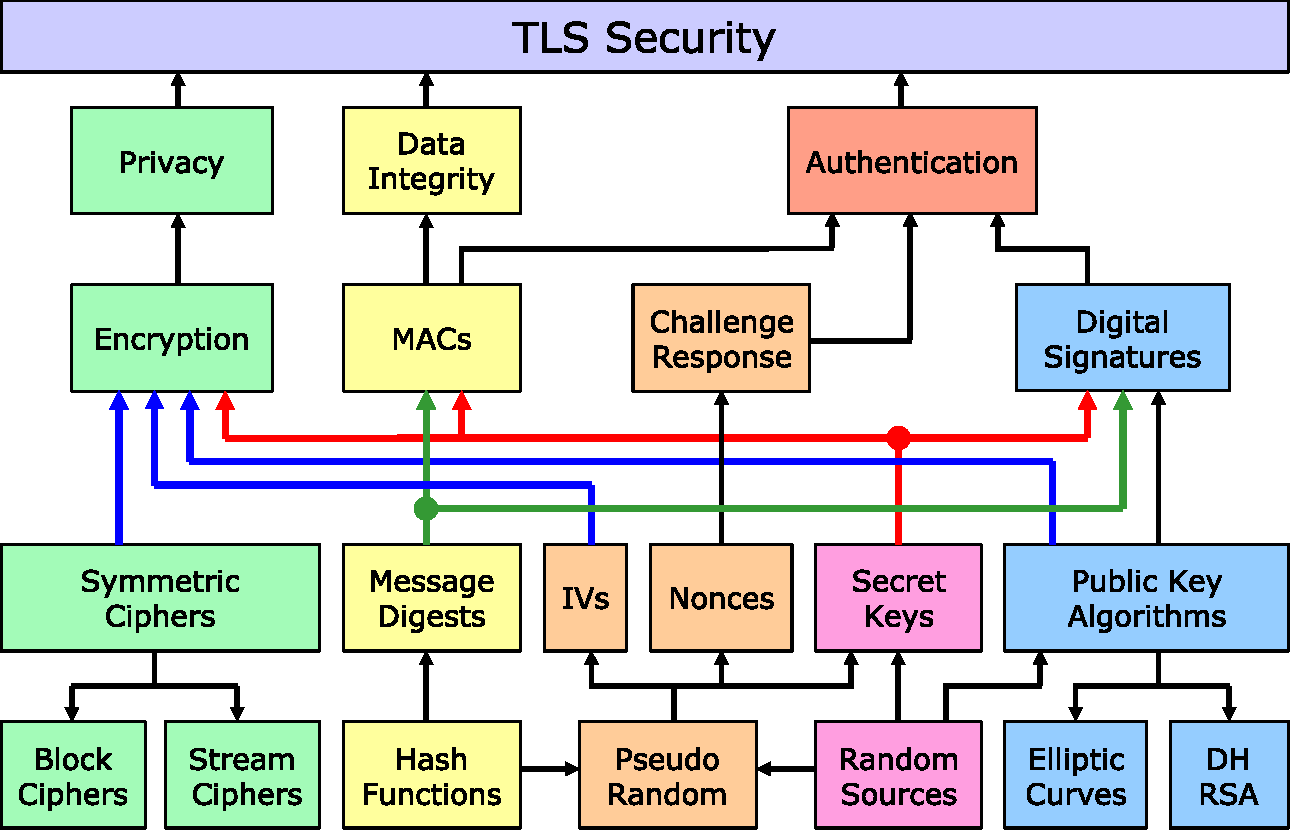
\includegraphics[width=\textwidth]{fig/crypto_blocks}
    \caption{Ferramentas criptográficas e suas inter-correlações}
    \label{fig:crypto_blocks}
\end{figure}

Como ainda não há um consenso na tradução para português de alguns termos 
básicos em criptografia, arbitramos pela seguinte terminologia nesse 
documento:

\begin{center}
    \begin{tabular}{@{}ll@{}} \toprule
	\tm{Inglês} & \tm{Português} \\ \midrule
encryption & cifragem \\
decryption & decifragem \\
cipher & cifrador \\
plaintext & mensagem ou texto legível \\
ciphertext & texto cifrado \\ \bottomrule
    \end{tabular}
\end{center}

Nas descrições dos algoritmos empregaremos a simbologia expressa na Tabela~\vref{tab:simbologiaAlgoritmos}.

\begin{table}[htbp]
	\centering
		\caption{Simbologia usada nas definições dos algoritmos}
		\begin{tabular}{@{}cl@{}} \toprule
		\tm{Símbolo} & \tm{Significado} \\ \midrule
		$m$ 						& Texto legível ou mensagem. \\
		$c$							& Texto cifrado. \\
		$h, i, r, s, v$				& Outros resultados/textos. \\
		\textsf{A} 					& Entidade origem. \\
		\textsf{B} 					& Entidade destino. \\
		$D, E, H, I, S, V$ 			& Funções/transformações. \\
		$\delta, \varepsilon, \kappa$ 	& Chaves criptográficas. \\
		
\includegraphics[scale=0.5]{fig/secret_key} & Chave secreta ($\kappa$). \\
		
\includegraphics[scale=0.5]{fig/public_key} & Chave pública ($\delta$) da entidade ``E''. \\
		
\includegraphics[scale=0.5]{fig/private_key} & Chave privada ($\varepsilon$) da entidade ``E''. \\ \bottomrule
		\end{tabular}
	\label{tab:simbologiaAlgoritmos}
\end{table}

\section{Funções de \emph{Hash} (resumo criptográfico)}

Uma Função de \emph{Hash} $H$ retorna, para uma mensagem $m$ de tamanho arbitrário 
qualquer, uma seqüência de bytes $h$ de tamanho fixo, chamada valor de \emph{hash} ou 
resumo criptográfico. Mais precisamente:
\[ h = H(m) \]
%Uma Função de \emph{Hash} criptograficamente segura deve apresentar as
%seguintes propriedades:

%\begin{description}
%    \item[Unidirecional] -- Encontrar $m = H^{-1}(h)$ deve ser
%    computacionalmente impraticável;
%    \item[Fracamente Livre de Colisões] -- Dada uma mensagem $m_1$, encontrar
%    $m_2$ diferente de $m_1$ tal que $H(m_1) = H(m_2)$ deve ser computacionalmente
%    impraticável;
%    \item[Fortemente Livre de Colisões] -- Encontrar $m_1$ e $m_2$ quaisquer
%    tal que $H(m_1) = H(m_2)$ deve ser computacionalmente impraticável.
%\end{description}
Dentre as diversas funções de \emph{Hash} existentes, o TLS limita-se aos algoritmos \acs{MD5} \cite{rfc_md5} e 
\acs{SHA1} \cite{fips_sha1}, cujos resumos são de 16 e 20 bytes respectivamente.

O valor de \emph{hash} quando representa a mensagem da qual derivou é chamado
de \emph{message digest}.

\section{Algoritmos de Chave Secreta}

Os algoritmos de chave secreta (\aclp{SKA} ou \acsp{SKA}) se caracterizam pela utilização de uma mesma chave para as 
operações complementares (cifrar/decifrar ou assinar/verificar).

A segura utilização destes algoritmos demanda, entretanto, pela solução de três problemas intrínsecos:

\begin{enumerate}
\item A distribuição confidencial da chave secreta entre duas entidades que precisa ser
efetuada \emph{a priori} por (outro) canal seguro;
\item O crescimento exponencial, da ordem de $O(n^2)$\footnote{A rigor: 
$\lim_{n \to \infty} \frac{n (n - 1)}{2} = n^2$},
da quantidade de chaves em função do número de entidades envolvidas ($n$)\footnote{Assumindo 
que será utilizada uma chave única para cada par de entidades.};
\item Como a sigilosidade de uma chave secreta decai na medida em que aumenta a sua exposição, torna-se
imperativo portanto que esta chave secreta tenha um curto ciclo de vida, requisito este difícil de 
ser atendido, considerando-se os dois problemas citados acima.
\end{enumerate}

No TLS, assim como em outros criptossistemas, esses problemas são resolvidos com o uso de
algoritmos de chave pública (ver seção~\ref{sec:pk}).

\subsection{\acl{MAC}}

O código de autenticação de mensagem (\acs{MAC}), também chamado de \ac{MIC},
é uma especialidade de resumo criptográfico computado em função
da mensagem $m$ e de uma chave secreta $\kappa$. A autenticidade da origem e a
integridade da mensagem podem ser comprovadas pelo destinatário usando-se a
mesma chave $\kappa$, como ilustra a Figura~\vref{fig:sk_sign}, na qual o
algoritmo de MAC/MIC está simbolizado pela função $I$ e o resumo por $i$.

\begin{figure}[htbp]
	\centering
		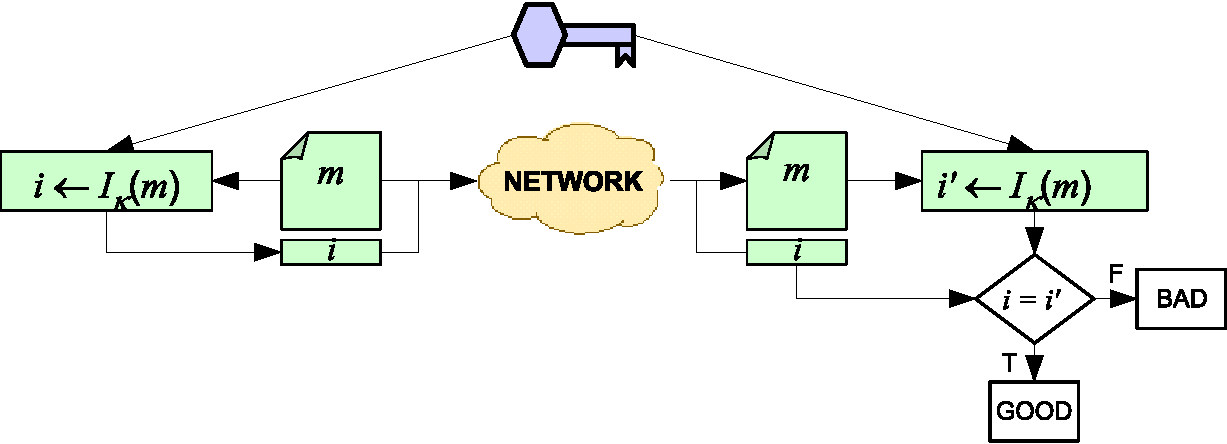
\includegraphics[scale=0.7]{fig/sk_sign}
	\caption{Geração e validação do MAC}
	\label{fig:sk_sign}
\end{figure}

Dentre os diversos tipos de \acs{MAC} já elaborados, o único
utilizado no TLS é o baseado em funções \emph{Hash}, mais precisamente o \ac{HMAC}
especificado em \cite{rfc_hmac} e que pode ser resumido na seguinte equação:
\[ i = HMAC_\kappa(H,m) = H(\kappa \oplus \mathtt{opad} \;\|\; H(\kappa \oplus \mathtt{ipad} \;\|\; m)) \]
onde:

\begin{tabular}{@{}rp{13cm}@{}}
$H(a)$		& Uma função de \emph{Hash} qualquer aplicada à seqüência $a$.
		  		  No caso do TLS, $H$ está limitado a \acs{MD5} ou \acs{SHA1}. \\
\addlinespace
$\kappa$	& Chave secreta com 64 bytes completada com zeros à direita. \\
\addlinespace
$\|$		& Operador de concatenação de seqüências. \\
\addlinespace
$\oplus$	& Operador binário OU-Exclusivo. \\
\addlinespace
$\mathtt{ipad}$ & O byte \texttt{0x36} repetido 64 vezes. \\
\addlinespace
$\mathtt{opad}$ & O byte \texttt{0x5C} repetido 64 vezes. \\
\end{tabular}

\subsection{Cifradores Simétricos}

Os cifradores simétricos utilizam a mesma chave $\kappa$ para o processo de cifragem ($E_\kappa$) 
e decifragem ($D_\kappa \equiv E_\kappa^{-1}$), conforme ilustra a Figura \vref{fig:sk_encryption}.

	\begin{figure}[htbp]
		\centering
			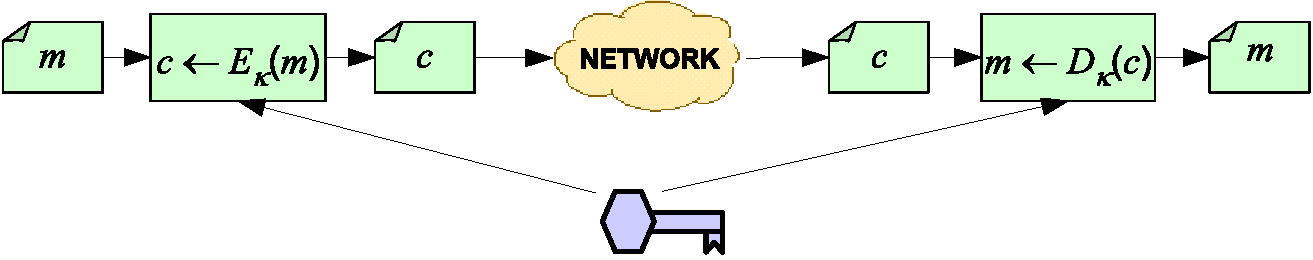
\includegraphics[scale=0.7]{fig/sk_cipher}
		\caption{Cifragem e decifragem usando SKA}
		\label{fig:sk_encryption}
	\end{figure}

Cifradores simétricos são normalmente classificados em seqüenciais
(\emph{stream ciphers}), que cifram/decifram um byte por vez, ou cifradores de
bloco (\emph{block ciphers}), que atuam sobre blocos de tamanho fixo,
usualmente 8 ou 16 bytes.

Dentre os cifradores simétricos oficialmente suportados pelo TLS, o único 
seqüencial é o RC4 \cite{rfc_rc4}. Os demais cifradores (de bloco) relacionados na norma são 
DES \cite{fips_des}, Triple-DES \cite{ansi_3des}, RC2 \cite{rfc_rc2} e IDEA \cite{idea}, que usam blocos de 8 bytes.

\section{Algoritmos de Chave Pública}
\label{sec:pk}

Os algoritmos de chave pública (\aclp{PKA} ou \acsp{PKA}) usam um par de chaves
matematicamente complementares, sendo uma delas tornada pública (doravante denotada por $\delta$) 
e a outra, chamada chave privada (simbolizada por $\varepsilon$), que deve ser conhecida apenas pela entidade
proprietária.

Esses algoritmos apresentam uma solução simples e revolucionária para o problema de distribuição de chaves, 
já que as chaves públicas não precisam trafegar por canais confidenciais. No entanto, a autenticidade da
origem das chaves e a integridade destas precisam estar asseguradas (ver seção \ref{sec:certs}).

Como é necessário distribuir apenas uma chave por entidade, os \acsp{PKA} estão naturalmente isentos do
segundo problema apresentado pelos \acsp{SKA}, já que o crescimento da quantidade de chaves é linear.

Em função de sua maior complexidade computacional, os \acsp{PKA} são tipicamente 10.000 vezes mais lentos
que os \acsp{SKA}. O TLS emprega então um criptossistema híbrido
onde os \acsp{SKA} são usados para os serviços de confidencialidade e integridade, com chaves secretas dinâmicas
estabelecidas através de \acsp{PKA}, que são também empregados para o serviço de autenticidade da origem e
assinatura digital.

Os \acsp{PKA} são tradicionalmente classificados conforme as seguintes propriedades~\cite{pki_book}:
cifragem , assinatura digital e estabelecimento de chave. 

\subsection{Cifragem}

Quando é reversível, ou seja, as duas transformações (denotadas por $E$ e $D$) são inversas entre si.

\begin{figure}[htbp]
	\centering
		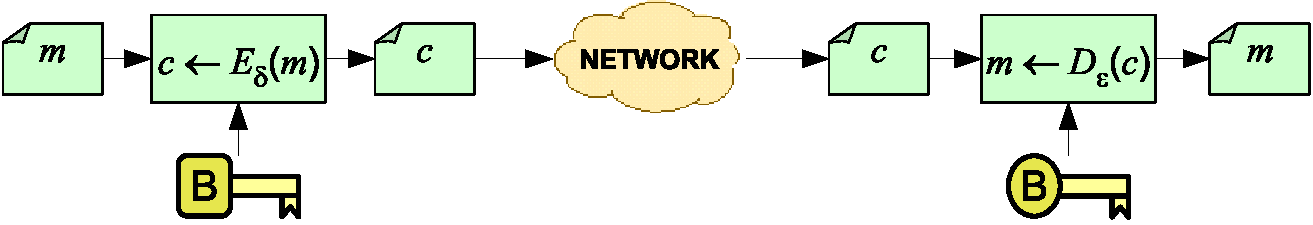
\includegraphics[scale=0.7]{fig/pk_cipher}
	\caption{Cifragem e decifragem com PKA}
	\label{fig:pk_encryption}
\end{figure}

O único algoritmo reversível oficializado na norma é o \acs{RSA} \cite{rsa}.

\subsection{Assinatura Digital}

Quando a sua chave privada pode ser utilizada por uma transformação $S_\varepsilon$
para a geração de um resumo especial (a ``assinatura'') 
a partir da texto legível. Este resumo será usado pela entidade destino que, com o uso da chave pública
da entidade origem e da função complementar $V_\delta$, poderá comprovar 
autenticidade e integridade da mensagem recebida.

\begin{figure}[htbp]
	\centering
		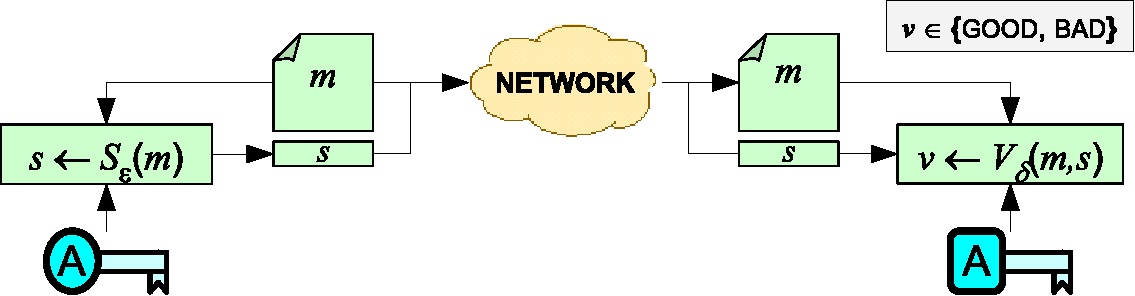
\includegraphics[scale=0.7]{fig/pk_sign}
	\caption{Assinatura Digital com PKA}
	\label{fig:pk_sign}
\end{figure}

A norma TLS especifica os algoritmos \ac{DSS} \cite{fips_dss} e o \acs{RSA} que, por ser reversível, pode ser 
usado aplicando-se as seguintes relações de equivalência:
\begin{eqnarray}
S_\varepsilon(m) & \equiv & E_\varepsilon(H(m)) \nonumber \\
V_\delta(m,s) & \equiv & D_\delta(s) \stackrel{?}{=} H(m) \nonumber
\end{eqnarray}

\subsection{Estabelecimento de Chave}

Quando o \acs{PKA} pode ser usado para a criação de um protocolo que permite o
compartilhamento de uma chave secreta entre as duas entidades participantes,
mas ainda assim confidencial. Existem dois métodos para este fim:
\begin{description}
	\item[Transferência] -- Uma das entidades é responsável pela geração da chave secreta que
	é enviada para a outra entidade após ser cifrada com chave pública desta, garantindo assim a
	confidencialidade da transferência.
	O PKA utilizado nesse caso deve ser obviamente reversível, como por exemplo o \acs{RSA}.
	\item[Comum Acordo] -- As duas entidades contribuem conjuntamente para a geração da chave secreta utilizando
	somente parâmetros criptográficos públicos, incluindo as chaves públicas de ambas as entidades.
	O \ac{DH} \cite{dh76} é um exemplo típico de algoritmo dessa categoria.
\end{description}

\section{Certificados Digitais}
\label{sec:certs}

No TLS todas as chaves públicas (PKs) devem ser armazenadas e distribuídas em certificados digitais
segundo o formato \acs{ITUT} X.509 versão 3 \cite{rfc_x509}. A principal finalidade de um
certificado é vincular uma chave pública à uma entidade final, conhecedora da respectiva
chave privada, e identificada por um nome universalmente único, denominado \acf{DN}.

A confiança na veracidade dessa associação é garantida pela assinatura digital emitida
por uma entidade confiável \emph{a priori}, chamada Autoridade Certificadora ou \ac{CA}.

Um certificado contém basicamente as seguintes informações:

\begin{itemize}
	\item DN da entidade final;
	\item PK correspondente com todos os seus parâmetros criptográficos necessários,
	junto com uma identificação do algoritmo (\acs{RSA} ou \acs{DSS});
	\item Período de validade;
	\item DN da CA emissora;
	\item Assinatura digital emitida pela \acs{CA}.
\end{itemize}

Um certificado contém também a definição sobre a política de utilização da PK nele contida,
se esta pode ou não ser utilizada para assinar outros certificados.

Quanto à política de utilização da sua PK e o tipo de assinatura do seu certificado,
as entidades são normalmente classificadas em três categorias:

\begin{center}
	\begin{tabular}{@{}lp{6cm}p{5cm}@{}} \toprule
		\tm{Tipo de} & \tm{Uso da PK}  	& \tm{Assinatura do} \\
		\tm{Entidade}&					& \tm{seu certificado} \\ \midrule
		Entidade final & Pode ser usada para qualquer propósito
						 \underline{exceto} para a assinatura digital. & Assinado por uma CA. \\
		CA Intermediária & Somente para a assinatura digital de outros certificados & Assinado por outra CA. \\
		CA Raiz			 & Idem & Auto-assinado. \\ \bottomrule
	\end{tabular}
\end{center}

A seqüência de certificados:
\[ C_0, C_1, C_2, \ldots, C_n \]

onde:

\begin{center}
	\begin{tabular}{@{}rl@{}}
		$C_0$ & Certificado da CA raiz, ou seja, auto-assinado. \\
		$C_1,\ldots,C_{n-1}$ & Certificados das CAs Intermediárias. \\
		$C_n$ & Certificado da entidade final. \\
	\end{tabular}
\end{center}

é chamada caminho de certificação (\emph{``Certification Path''}) da entidade final associada ao certificado $C_n$.

%%%%%%%%%%%%%%%%%%%%%%%%%%%%%%%%%%%%%%%%%%%%%
%% Introdução ao protocolo TLS
%% Copyright 2006 Eliézio Batista de Oliveira
%%%%%%%%%%%%%%%%%%%%%%%%%%%%%%%%%%%%%%%%%%%%%

\chapter{Introdução ao protocolo TLS}

É apresentada a seguir uma descrição básica do protocolo TLS. Uma descrição
completa do protocolo pode ser encontrada na especificação
oficial~\cite{rfc_tls} ou mais detalhadamente no livro \emph{``SSL and
TLS: Designing and Building Secure Systems''}~\cite{Rescorla}.

\section{O criptossistema TLS}
\label{sec:OCriptossistemaTLS}

O TLS é um criptossistema híbrido onde todos os parâmetros dos algoritmos 
simétricos são dinâmicos e derivados de um parâmetro-mestre chamado \emph{master-key},
por sua vez definido através de um \acs{PKA} para o estabelecimento de chave.

No TLS os algoritmos criptográficos não podem ser combinados livremente mas
são pré-arranjados em forma de \emph{ciphersuites}.
Um \emph{ciphersuite} é basicamente uma quádrupla $<Au,Kx,Enc,Mac>$ que denota
respectivamente os algoritmos de autenticação, de estabelecimento de chave, 
de cifragem e a função de \emph{Hashing} usado no cômputo do \acs{HMAC}.

\section{Conexão e Sessão TLS}
\label{sec:ConexãoESessãoTLS}

Uma conexão TLS é um canal transiente estabelecido entre duas aplicações tendo por base 
um protocolo de transporte confiável, tipicamente o \acs{TCP}. Uma conexão tem
fundamentalmente duas fases distintas: \emph{handshake} e transferência de dados
das aplicações (\emph{bulk data transfer}).

O \emph{handshake} TLS possui três propósitos:
\begin{enumerate}
	\item Negociar o \emph{ciphersuite} e os parâmetros da sessão TLS (definida abaixo);
	\item Derivar todos os demais parâmetros criptográficos usados pelos algoritmos 
	simétricos;
	\item Autenticar as partes envolvidas (opcional).
\end{enumerate}

Uma sessão TLS é caracterizada pelos seguintes atributos:

\begin{center}
\begin{tabular}{@{}rp{10cm}@{}} \toprule
	\tm{Version} 		& Versão do protocolo TLS ou SSL. \\
	\addlinespace
	\tm{Session ID} 	& Identificador da sessão, definido pelo servidor. \\
	\addlinespace
	\tm{master-key}		& Chave mestre definida através de um \acs{PKA} para
	o estabelecimento de chave. \\
	\addlinespace
	$<Enc,Mac>$			& Algoritmos de cifragem e MAC, subconjunto do \emph{ciphersuite}. \\
	\addlinespace
	\tm{Compression Method} & Algoritmo de compressão. \\ \bottomrule
\end{tabular}
\end{center}

Uma vez constituída, uma sessão pode ser restaurada nas conexões subseqüentes, economizando
assim o alto custo computacional exigido para seu estabelecimento.

\section{Arquitetura do protocolo TLS}
\label{sec:ArquiteturaDoProtocoloTLS}

O TLS é implementado de modo a atuar entre a camada de aplicação e a de
transporte, como ilustra a Figura~\vref{fig:tls_stack} adaptada
de~\cite{Thomas}.

\begin{figure}[htbp]
    \centering
        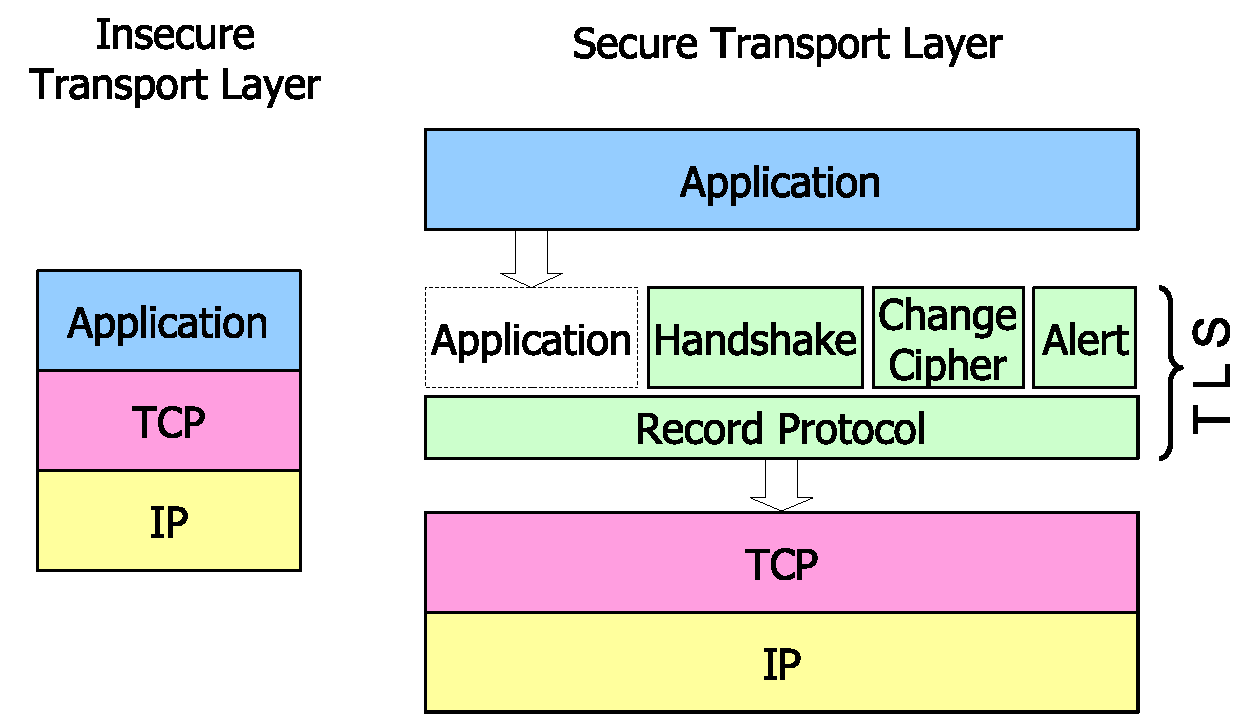
\includegraphics[scale=0.5]{fig/tls_stack}
    \caption{TLS na arquitetura em camadas de protocolos}
    \label{fig:tls_stack}
\end{figure}

O TLS pode ser decomposto em quatro sub-protocolos dispostos em duas camadas,
sendo um inferior, chamado de \emph{Record Protocol} e três superiores a saber:
\emph{Handshake}, \emph{Alert} e \emph{Change Cipher Spec} (CCS).

Do ponto de vista funcional, o CCS, composto de uma única mensagem homônima, é
parte integrante do \emph{handshake} e assim será abordado neste texto. A sua
discriminação como um protocolo em separado serve apenas ao único propósito de
garantir que a sua mensagem não compartilhe o mesmo registro com as demais
mensagens do \emph{handshake}.

\subsection{\emph{TLS Record Protocol}}

Um registro TLS encapsula uma ou mais mensagens recebidas de um dos
quatro protocolos superiores, e processadas conforme os mesmos parâmetros 
criptográficos correntes na conexão TLS. 

Conforme exposto na Figura~\vref{fig:tls_rec_protocol},
toda mensagem oriunda das camadas superiores é primeiramente
fragmentada em blocos de até $2^{14}$ bytes (16 kB), sendo eventualmente
comprimida em seguida\footnote{A RFC~2246 não especifica nenhum
algoritmo de compressão.}.

\begin{figure}[htbp]
    \centering
        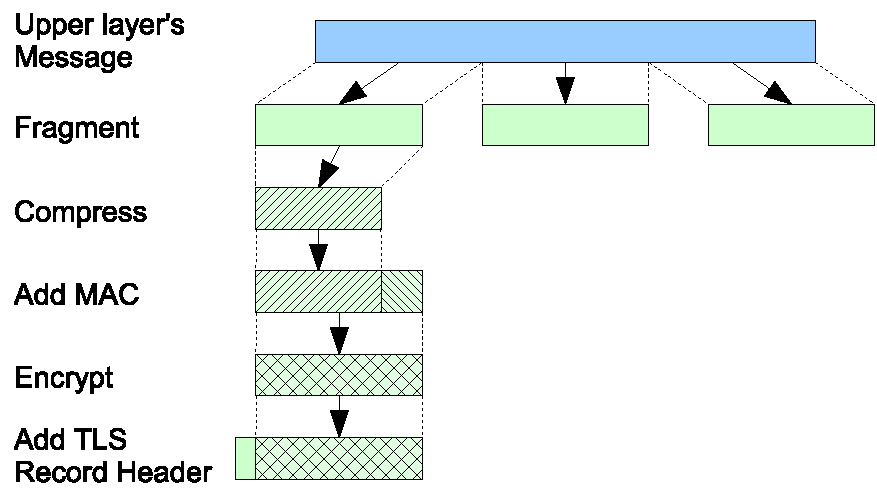
\includegraphics[scale=0.7]{fig/tls_rec_protocol}
    \caption{\emph{TLS Record Protocol}}
    \label{fig:tls_rec_protocol}
\end{figure}

O próximo estágio no processamento da mensagem é o cálculo e o acréscimo do seu
\acs{MAC}, provendo assim a verificabilidade da integridade da mensagem e da
autenticidade da sua origem.

Se o cifrador corrente for do tipo \emph{block cipher}, acrescenta-se tantos
bytes extras quanto forem necessários até que a soma do fragmento comprimido mais
o MAC seja um múltiplo inteiro do tamanho do bloco do cifrador.

Finalmente ocorre a cifragem de toda a mensagem concatenada ao seu \acs{MAC}
usando um cifrador simétrico, sendo em seguida prefixada por um \emph{header}
de cinco bytes ilustrado na Figura~\vref{fig:tls_rec_header} e descrito na Tabela~\vref{tab:TLSRecordHeader}.

\begin{figure}[htbp]
	\centering
		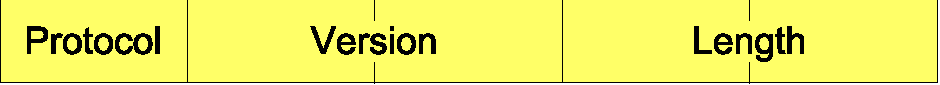
\includegraphics[scale=0.4]{fig/tls_rec_header}
	\caption{\emph{TLS Record Header}}
	\label{fig:tls_rec_header}
\end{figure}

\begin{table}[htbp]
	\centering
		\begin{tabular}{@{}lcp{10cm}@{}} \toprule
		\tm{Campo} & \tm{Tamanho} & \tm{Descrição} \\ \midrule
		\emph{Protocol} & 1 & Indica o protocolo superior das mensagens encapsuladas
						 segundo a seguinte codificação:
						\begin{center}
						\begin{tabular}{@{}cl@{}}
						 \tm{Tipo} & \tm{Protocolo} \\ \midrule
							20 & \tlsHsCcs \\
							21 & \emph{Alert} \\
							22 & \emph{Handshake} \\
							23 & \emph{Application Data} \\
						\end{tabular}
						\end{center} \\
		\emph{Version} & 2 & Versão do protocolo. A versão 1.0 do TLS é codificada 
							 como \verb|03 01| (em hexadecimal). \\
		\addlinespace
		\emph{Length}  & 2 & Tamanho total do conteúdo do registro, não podendo exceder a $2^{14} + 2048$. \\ \bottomrule
		\end{tabular}
	\caption{\emph{TLS Record Header}}
	\label{tab:TLSRecordHeader}
\end{table}

O \emph{ciphersuite} ativo no início de uma conexão é o $<NULL,NULL,NULL,NULL>$.

\subsection{\emph{Alert Protocol}}

A única mensagem que compõe esse protocolo pode ser enviada assincronamente por 
qualquer uma das partes para notificar erros para o outro par.

\subsection{\emph{Handshake Protocol}}

O \emph{handshake}, por ser o estágio certamente mais complexo, será analisado
mais detalhadamente a seguir através da análise de três casos típicos.

Para evitar aspectos do protocolo TLS desnecessários tendo em vista o escopo 
deste projeto, o \acs{RSA} será o PKA para o estabelecimento de chave empregado
em todos os \emph{handshakes} que se seguem.

\subsubsection{\emph{Handshake} com autenticação do servidor}

A autenticação do servidor é realizada em praticamente todas as negociações
TLS. A Tabela~\vref{tab:hs_server_auth} sumariza cada uma das mensagens
exibidas na Figura~\ref{fig:hs_server_auth}.


\begin{figure}[htp]
    \centering
        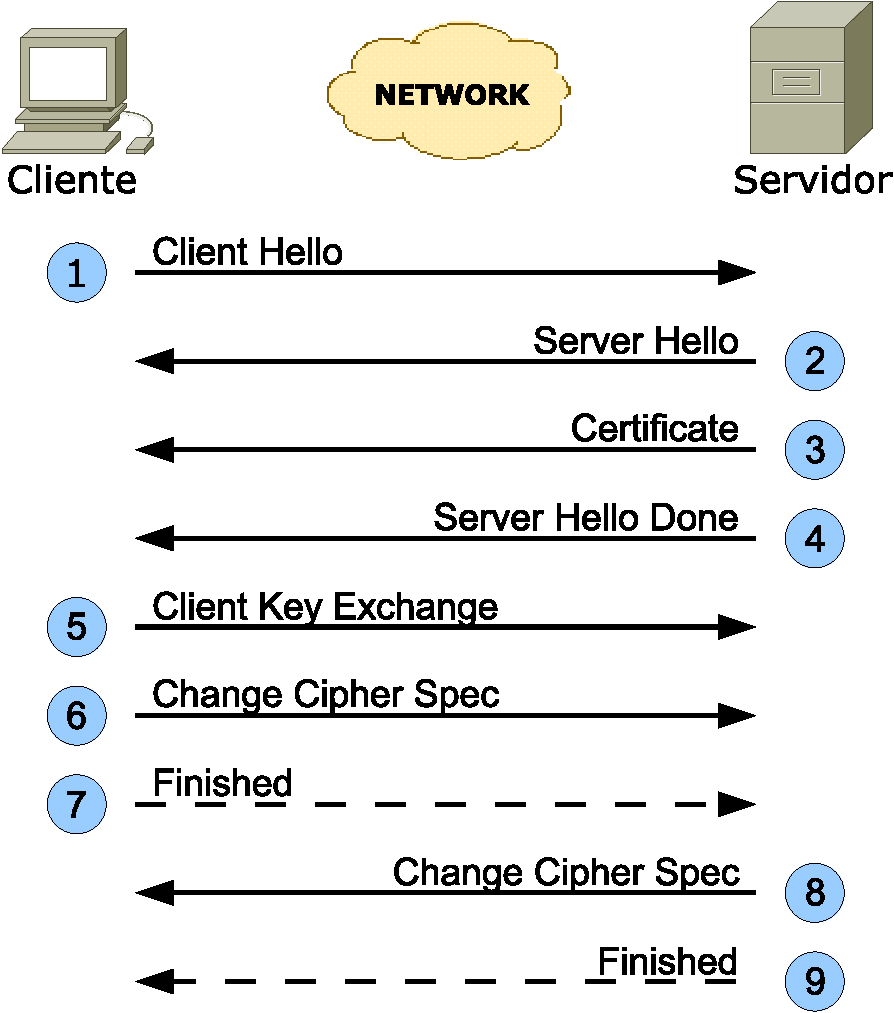
\includegraphics[scale=0.5]{fig/hs_server_auth}
    \caption{\emph{Handshake} completo com autenticação do servidor}
    \label{fig:hs_server_auth}
\end{figure}

\begin{table}[htp]
    \begin{center}
    \caption{\emph{Handshake} completo com autenticação do servidor}
    \label{tab:hs_server_auth}
    \begin{tabular}{@{}lp{15cm}@{}} \toprule
        \tm{\#} & \tm{Descrição} \\ \midrule
1 &
O cliente envia a mensagem \tlsHsCh propondo os seguintes parâmetros
para a conexão:
\begin{itemize}
\item \emph{Version} -- Versão máxima do protocolo suportada (3.1 para o caso do
TLS 1.0);
\item \emph{Nonce} -- Um número (pseudo-) aleatório de 32 bytes recém gerado
para esta conexão;
\item \emph{Session ID} -- Identificador de uma sessão previamente estabelecida,
caso o cliente deseje restaurá-la;
\item \emph{Cipher Suites} -- Lista dos parâmetros criptográficos suportados pelo
cliente;
\item \emph{Compression Methods} -- Lista dos métodos de compressão suportados.
\end{itemize} \\

2 &
Servidor responde com \tlsHsSh selecionando os parâmetros dentre
aqueles propostos pelo cliente e incluindo o seu próprio \emph{Nonce}. \\
\addlinespace
3 &
Servidor envia seu certificado e todos os intermediários que porventura
existam. \\
\addlinespace
4 &
O servidor conclui esse primeiro estágio de negociação com a mensagem
\tlsHsShd. \\
\addlinespace
5 &
O cliente gera uma chave de sessão aleatória e a envia cifrada com a chave
pública do servidor na mensagem \tlsHsCke. \\
\addlinespace
6 &
Através da mensagem \tlsHsCcs o cliente efetiva os parâmetros
criptográficos já acordados. Todas as mensagens subseqüentes passam a ser
cifradas conforme esses novos parâmetros. \\
\addlinespace
7 &
Um \emph{hash} de todas as mensagens enviadas e recebidas é enviado para o
servidor para evitar que negociação não sofra nenhuma interferência
indevida. \\
\addlinespace
8 &
O servidor também efetiva os parâmetros recém-negociados. \\
\addlinespace
9 &
O servidor envia o \emph{hash} calculado sobre as mensagens enviadas e recebidas
para reforçar a integridade da negociação. \\ \bottomrule
    \end{tabular}
    \end{center}
\end{table}

\subsubsection{\emph{Handshake} com autenticação mútua}

\begin{figure}[htp]
    \centering
        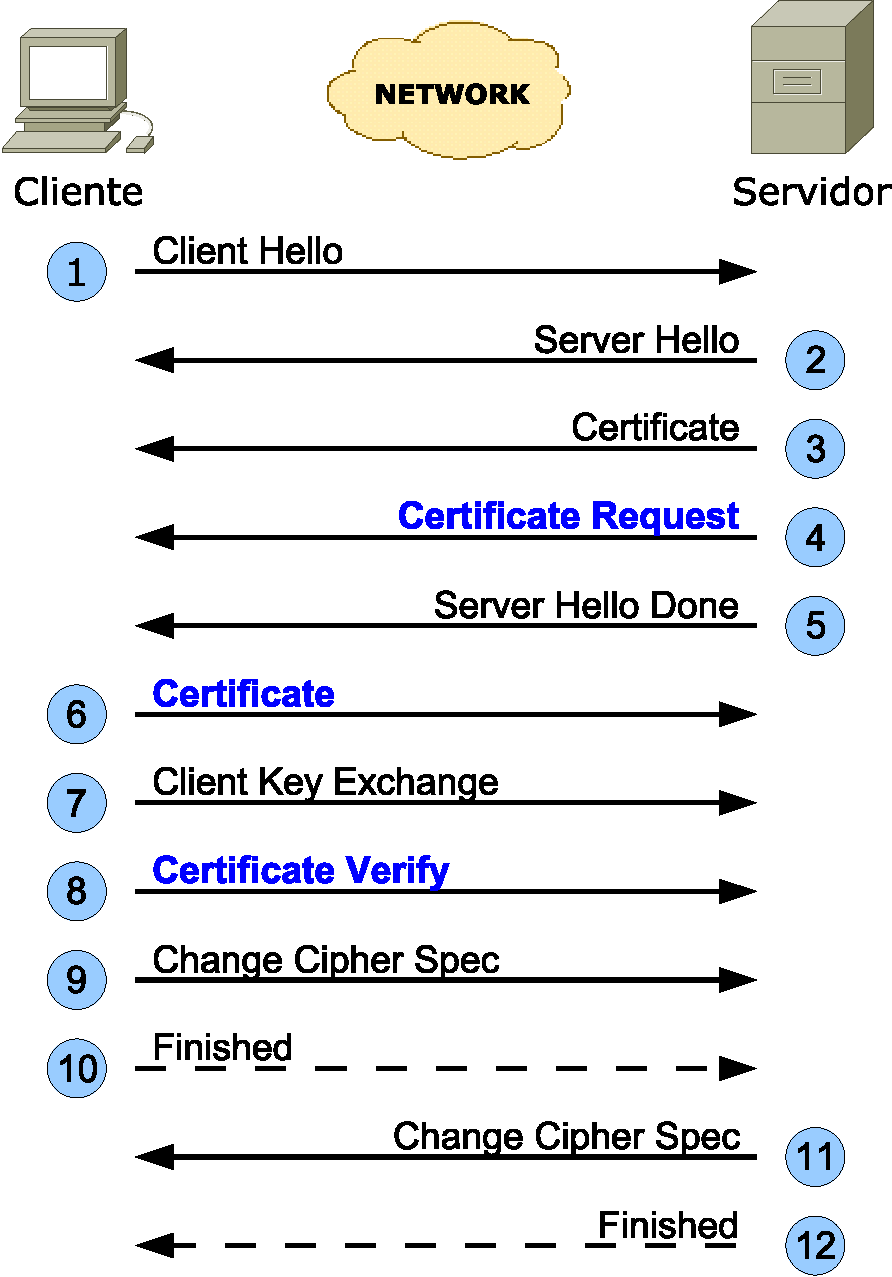
\includegraphics[scale=0.5]{fig/hs_mutual_auth}
    \caption{\emph{Handshake} completo com autenticação mútua}
    \label{fig:hs_mutual_auth}
\end{figure}

A Tabela~\vref{tab:hs_mutual_auth} resume as mensagens adicionais destacadas em negrito na
Figura~\vref{fig:hs_mutual_auth}.

\begin{table}[htp]
    \begin{center}
    \caption{\emph{Handshake} completo com autenticação mútua}
    \label{tab:hs_mutual_auth}
    \begin{tabular}{@{}cp{15cm}@{}} \toprule
    \tm{\#} & \tm{Descrição} \\ \midrule
4 &
O servidor solicita ao cliente que envie o seu certificado X.509. A mensagem
\tlsHsCr inclui uma lista das \acsp{CA} aceitáveis pelo servidor. \\
\addlinespace
6 &
O cliente envia o seu certificado e todos os eventuais certificados
intermediários (não raiz). \\
\addlinespace
8 &
Adicionalmente o cliente precisa enviar uma prova de autenticidade,
comprovando que possui a chave privada correspondente à chave pública
incluída no seu certificado. \\ \bottomrule
    \end{tabular}
    \end{center}
\end{table}

\subsubsection{\emph{Handshake} abreviado}

Esse mecanismo, denominado pela especificação de \emph{Session Resumption},
permite a restauração de uma sessão TLS negociada anteriormente, reduzindo todo
o \emph{handshake} a apenas 6 breves mensagens e dispensando todo esforço
computacional necessário para estabelecer uma nova conexão TLS. A
Tabela~\vref{tab:hs_resumed} descreve as principais mensagens que determinam a
restauração de uma sessão, cujo processo completo encontra-se ilustrado na
Figura~\vref{fig:hs_resumed}.

\begin{figure}[htb]
    \centering
        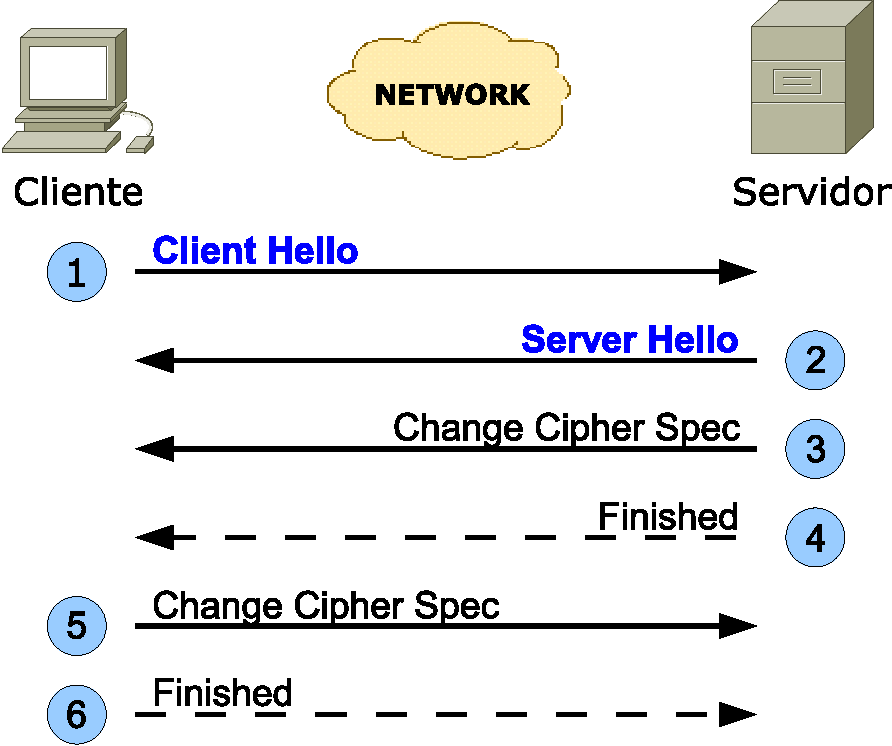
\includegraphics[scale=0.50]{fig/hs_resumed}
    \caption{\emph{Handshake} abreviado}
    \label{fig:hs_resumed}
\end{figure}

\begin{table}[htp]
    \centering
    \caption{\emph{Handshake} abreviado}
    \label{tab:hs_resumed}
    \begin{tabular}{@{}lp{15cm}@{}} \toprule
        \tm{\#} & \tm{Descrição} \\ \midrule
1 &
O cliente envia a mensagem \tlsHsCh contendo todos os parâmetros necessários para o
estabelecimento de uma nova sessão, mas inclui o identificador de sessão (\emph{``Session ID''}) extraído
da \tlsHsSh enviada por este servidor em uma sessão anterior. \\
\addlinespace
2 &
Servidor responde com \tlsHsSh contendo o mesmo identificador presente na \tlsHsCh, sinalizando
que a sessão será restaurada. \\ \bottomrule
    \end{tabular}
\end{table}

%%%%%%%%%%%%%%%%%%%%%%%%%%%%%%%%%%%%%%%%%%%%%
%% Introdução a RFC 3546
%% Copyright 2006 Eliézio Batista de Oliveira
%%%%%%%%%%%%%%%%%%%%%%%%%%%%%%%%%%%%%%%%%%%%%

\chapter{As extensões do protocolo TLS}

As recomendações presentes na RFC 3546 podem ser desmembradas em duas 
partes distintas. A primeira trata da especificação de um mecanismo genérico 
de codificação e negociação das extensões ao TLS. A segunda parte especifica
6 extensões que, em geral, visam reduzir o \emph{overhead} do protocolo TLS.

As extensões codificadas devem ser acrescentadas ao final das mensagens 
\tlsHsCh e \tlsHsSh. Essa abordagem permite a compatibilidade com 
as implementações de TLS pré-existentes, uma vez que a sua 
especificação determina claramente que (\rfcurl{2246}{7.4.1.2}):
 
\begin{quote}
{\smaller
\begin{verbatim}
Forward compatibility note: 
    In the interests of forward compatibility, it is permitted for a 
    client hello message to include extra data after the compression 
    methods. This data must be included in the handshake hashes, but 
    must otherwise be ignored. This is the only handshake message for 
    which this is legal; for all other messages, the amount of data 
    in the message must match the description of the message 
    precisely.
\end{verbatim}
}
\end{quote}

As principais diretrizes na negociação das extensões são:

\begin{itemize}
\item Somente ao cliente é permitido propor extensões;
\item O servidor pode, para cada extensão proposta, tomar uma das seguintes ações:
\begin{enumerate}
    \item Aceitá-la e sinalizar essa aceitação acrescentando a mesma extensão
    ao \tlsHsSh;
    \item Ignorá-la silenciosamente;
    \item Rejeitá-la enviando uma mensagem \emph{Alert} para o cliente e
    abortando o \emph{handshake} imediatamente.
\end{enumerate}
\item Caso o servidor não confirme explicitamente a extensão proposta, o
cliente pode abortar a conexão caso julgue a extensão imprescindível.
\end{itemize}

A segunda parte da RFC~3546 propõe seis extensões específicas que acrescentam
novas funcionalidades ao protocolo TLS. Soma-se a elas uma sétima extensão
não-oficial especificada nesse documento e também implementada no OpenSSL.

Apresenta-se a seguir uma descrição sistemática de cada uma dessas extensões,
enfatizando os seguintes aspectos:

\begin{description}

\item[Referência] - Indica o trecho de documentação que contém os detalhes
técnicos sobre a extensão;

\item[Sinopse] - Um breve histórico da questão a ser resolvida e/ou aprimorada
pela extensão;

\item[Propósito da Extensão] - Descreve a solução proposta pela extensão;

\end{description}

\section{\acf{SNI}}

\begin{description}[\breaklabel]

\item[Referência]
	\rfcurl{3546}{3.1}.
	
\item[Sinopse]
	Servidores web, principalmente os comerciais, normalmente hospedam mais de um \emph{site}
	através de um mecanismo chamado \emph{name-based virtual hosting}, disponível em praticamente
	todos os servidores HTTP existentes. A seleção do domínio é feita pelo cliente HTTP (\emph{browser})
	através da campo `\verb|Host|' presente no \emph{request} HTTP \cite[seção~14.23]{rfc_http}.

	Nos servidores HTTPS a seleção do domínio precisa ser efetuada precocemente, pois é
	decisiva para a seleção do certificado do servidor a ser enviado, podendo também impactar na
	escolha de outros parâmetros da sessão.

	O campo `\verb|Host|' é, portanto, ineficiente para esta seleção uma vez que o \emph{request}
	HTTP é transmitido tardiamente, após a conclusão do \emph{handshake} TLS.

\item[Propósito da Extensão]
	A solução natural oferecida nesta extensão consiste na inclusão do nome do \emph{host} na primeira
	mensagem enviada pelo cliente, que é a \tlsHsCh.

\end{description}


\section{\acf{MFL}}

\begin{description}[\breaklabel]

\item[Referência]
	\rfcurl{3546}{3.2}.

\item[Sinopse]
	Na camada \emph{record layer}, cada registro recebido só pode ser disponibilizado
	para o protocolo superior após a verificação da sua integridade. Esse requisito
	obriga o cliente a dispor de memória suficiente para armazenar o maior registro 
	admitido pela especificação que é cerca de 16 kB.
	
\item[Propósito da Extensão]
	Essa extensão permite que o cliente estabeleça um limite superior para o tamanho de um 
	fragmento TLS, podendo variar de 512 até 4096 bytes.

\end{description}


\section{\acf{CCU}}

\begin{description}[\breaklabel]

\item[Referência]
	\rfcurl{3546}{3.3}.

\item[Sinopse]
	Sempre que a autenticação do cliente é solicitada pelo servidor, o cliente deve
	enviar uma mensagem \tlsHsC contendo um ou mais certificados.
	
\item[Propósito da Extensão]
	Com o uso dessa extensão, a mensagem \tlsHsC é substituída pela \tlsHsCu que
	conteria uma ou mais \acsp{URL} para a obtenção de toda a cadeia de certificados do 
	cliente.

\end{description}


\section{\acf{TCI}}

\begin{description}[\breaklabel]

\item[Referência]
	\rfcurl{3546}{3.4}.

\item[Sinopse]
	A princípio, um servidor pode estar configurado com mais de um certificado 
	para um mesmo \emph{Common Name} emitidos por \acsp{CA} diferentes.
	
\item[Propósito da Extensão]
	Essa extensão serviria então para informar ao servidor quais são os \acsp{CA} conhecidos e 
	confiáveis pelo cliente. O servidor teria então um critério para efetuar uma escolha 
	inequívoca sobre qual certificado X.509 deve empregado no \emph{handshake} TLS.

\end{description}


\section{\acf{TMAC}}

\begin{description}[\breaklabel]

\item[Referência]
	\rfcurl{3546}{3.5}.

\item[Sinopse]
	O MAC acrescentado a cada mensagem cifrada TLS, que pode ter 16 ou 20 bytes de tamanho
	conforme o algoritmo de \emph{Hash} em uso, pode representar uma parcela significativa
	nos dados trafegados, particularmente em comunicações interativas.

\item[Propósito da Extensão]
	Essa extensão permite que tanto cliente quanto servidor passem a usar um \acs{HMAC} reduzido 
	(truncado) a 10 bytes.

\end{description}


\section{\acf{CSR}}

\begin{description}[\breaklabel]

\item[Referência]
	\rfcurl{3546}{3.6}.

\item[Sinopse]
	O protocolo \ac{OCSP} \cite{rfc_ocsp} permite verificar em tempo real se um certificado foi 
	revogado ou não pelo \acs{CA} emissor.
	
\item[Propósito da Extensão]
	Com o uso dessa extensão, o servidor atuaria como um \emph{proxy} para a 
	obtenção de uma resposta \ac{OCSP} sobre o estado (revogado ou não-revogado) do 
	certificado do próprio servidor, dispensando assim o estabelecimento de uma segunda conexão TCP
	com o servidor (``\emph{responder}'') OCSP.
	
	O uso do \emph{proxy} seria benéfico também para os clientes que estivessem sujeitos a uma
	conectividade restrita, restrição comumente empregada em \acsp{VPN} para redes corporativas.

\end{description}


\section{\acf{SCCI}}

\begin{description}[\breaklabel]

\item[Referência]
	Draft em andamento. \\
	Autor: Eliézio Oliveira

\item[Sinopse]
	Como a cada novo \emph{handshake} TLS (portanto, sem \emph{``session resumption''}), o 
	servidor envia quase sempre a mesma seqüência de certificados, que 
	invariavelmente corresponde a maior parte do volume de dados trafegados, 
	decidimos acrescentar uma sétima extensão, a fim de evitar esse tráfego 
	redundante.

\item[Propósito da Extensão]
	Ao propor essa nova extensão, o cliente apresenta os identificadores de cada 
	certificado presente na cadeia de certificados previamente obtida. Esses 
	identificadores são exatamente os mesmos utilizados na extensão \acl{TCI}.

	Ao concordar com essa extensão, o servidor terá a opção de enviar uma 
	mensagem \tlsHsC vazia, mas ainda assim terá a alternativa de mandar a 
	cadeia inteira. O cliente deve, portanto, estar preparado para tratar os dois 
	casos ao processar a mensagem \tlsHsC enviada pelo servidor.

	Para eliminar qualquer possibilidade desta extensão deteriorar a segurança do 
	protocolo TLS, optou-se por incluir toda a seqüência de certificados no cômputo 
	do resumo criptográfico a ser publicado na mensagem \tlsHsF. Essa operação 
	deve ser efetuada imediatamente após a inclusão da mensagem \tlsHsC  
	recebida (cliente) ou enviada (servidor).

\end{description}



%%%%%%%%%%%%%%%%%%%%%%%%%%%%%%%%%%%%%%%%%%%%%
%% Implementação
%% Copyright 2006 Eliézio Batista de Oliveira
%%%%%%%%%%%%%%%%%%%%%%%%%%%%%%%%%%%%%%%%%%%%%

\chapter{Implementação das extensões}

\section{Diretrizes de desenvolvimento}

As extensões abordadas neste projeto foram implementadas como modificações 
no \emph{software} \emph{open-source} OpenSSL \cite{openssl}, versão 0.9.8a lançada em 11 de Outubro de 2005.
Recomendamos o livro \emph{``Network Security with OpenSSL''} \cite{opensslbook} que contém uma
extensa documentação da \acs{API} do OpenSSL, bem como guias de utilização das diversas
ferramentas que compõem o \emph{toolkit}.

O OpenSSL assim modificado foi testado com sucesso nas plataformas 
Microsoft Windows 2000 Professional e Linux/x86, mas acredita-se que não haverá 
problemas de portabilidade paras as outras dezenas de plataformas suportadas 
oficialmente pelo OpenSSL.

Optou-se por estender a \acs{API} do OpenSSL com 15 funções assim agrupadas:
\begin{itemize}
\item 12 funções a serem usadas pelo cliente TLS para selecionar e configurar as 
extensões que serão propostas na mensagem \tlsHsCh. Obviamente 
essas funções devem ser acionadas antes do início do \emph{handshake} TLS para 
que sejam efetivas;
\item 2 funções que se destinam a definir \emph{callbacks} no lado servidor para 
processar as extensões \acl{SNI} e \acl{CCU};
\item 1 função utilizável pelo servidor para indicar quais as extensões que 
serão reconhecidas e confirmadas.
\end{itemize}

Detalharemos a seguir cada uma das extensões implementadas, destacando os 
seguintes aspectos:

\begin{description}
\item[Especificação] -- Trecho relevante da especificação oficial para facilitar a 
comprovação da conformidade da implementação;
\item[Divergências] -- Pontos em que a implementação se desvia da
especificação;
\item[API Estendida] -- Detalhamento das funções específicas para aquela 
extensão;
\item[Implementação] -- Documentação das modificações realizadas no 
código-fonte do OpenSSL;
\item[Testes de Conformidade] -- \emph{Traces} de mensagens capturadas de testes 
reais que demonstram a eficácia da implementação e suas eventuais 
limitações.
\end{description}

Como um típico projeto \emph{open-source}, o OpenSSL não dispõe de uma documentação
sobre a sua arquitetura de \emph{software}. Uma breve descrição de algumas poucas estruturas
usadas internamente podem ser encontradas no capítulo \emph{``Advanced Programming Topics''} 
do livro \emph{``Network Security with OpenSSL''} supracitado.

\section{Modificações Gerais}

\subsection{\emph{Build}}

Todas as modificações feitas nos arquivos da distribuição oficial do OpenSSL 
foram condicionadas à definição da macro \verb|OPENSSL_NO_TLSEXT| que está
indefinida por default. Para defini-la, e conseqüentemente desabilitar todas as 
extensões, basta incluir a opção \verb|no-tlsext| na configuração do ambiente de 
\emph{build} do OpenSSL. Exemplo: \verb|./config no-tlsext| para as plataformas 
UNIX/Linux.

\subsection{Estruturas de Dados}

Foi criado um novo \emph{include header} \textit{``tlsx.h''} que, além de conter os protótipos 
das funções da \acs{API} estendida, define também a estrutura \verb|TLS_EXTENSIONS|
responsável por conter a representação das extensões a serem propostas e 
outras estruturas de dados necessárias para o processamento destas. Vide o Anexo~\ref{chap:tlsx_h}
para a definição completa desta estrutura.

Três das principais estruturas nativas do OpenSSL foram incrementadas para 
suportar as extensões alvo desse projeto:

\begin{description}[\breaklabel\setlabelstyle{\ttfamily}]

\item[ssl.h::SSL\_CTX, SSL]
	Inclusão do campo \verb|tlsx| (tipo: \verb|TLS_EXTENSIONS|) 
	contendo todas as estruturas necessárias durante o \emph{handshake}.

\item[ssl.h::SSL\_SESSION, ssl\_asn1.c::SSL\_SESSION\_ASN1]
	Incluídos 3 campos responsáveis pela representação de todas as informações que devem ser 
	persistidas junto com a sessão TLS, a saber: \verb|tlsx_servername|, 
	\verb|tlsx_max_fragment_length_id| e \verb|tlsx_truncated_hmac|.

\item[ssl3.h::SSL3\_STATE]
	Acrescentados os campos que representam os 
	parâmetros das 2 únicas extensões que impactam a conexão TLS após o 
	\emph{handshake}: \verb|tlsx_max_plain_length| e \verb|tlsx_truncated_hmac|.

\end{description}

\subsection{Funções Nativas}

Segue abaixo um resumo de todas as modificações genéricas efetuadas no 
código base do OpenSSL. As demais modificações específicas estão 
documentadas em cada extensão mais adiante.

\begin{description}[\breaklabel\setlabelstyle{\ttfamily}]

\item[s3\_clnt.c::ssl3\_client\_hello]
	Passou a chamar a função responsável pelo acréscimo das extensões 
	propostas (\verb|tlsx_write_request|) ao final da construção da mensagem 
	\tlsHsCh.

\item[s3\_clnt.c::ssl3\_get\_server\_hello]
	Chamada da nova função \verb|tlsx_read_response| para processar as respostas 
	do servidor TLS às extensões propostas, caso não tenha ocorrido uma 
	restauração da sessão.

\item[s3\_lib.c::ssl3\_clear]
	Modificada para restabelecer os valores default dos campos \verb|tlsx_max_plain_length| e 
	\verb|tlsx_truncated_hmac| da estrutura \verb|s3| (do tipo \verb|SSL3_STATE|), que são,
	respectivamente, \verb|SSL3_RT_MAX_PLAIN_LENGTH_DEFAULT| e \verb|FALSE|.

\item[s3\_srvr.c::ssl3\_get\_client\_hello]
	Em caso de nova sessão, chama a \verb|tlsx_read_request| para o 
	processamento das eventuais extensões.

\item[s3\_srvr.c::ssl3\_send\_server\_hello]
	Passou a chamar a \verb|tlsx_write_response| caso alguma extensão tenha sido 
	confirmada.

\item[ssl\_asn1.c::i2d\_SSL\_SESSION]
	Foi incrementada para cuidar da serialização em \acs{ASN1} dos três 
	parâmetros que devem ser persistidos: \verb|tlsx_servername|, 
	\verb|tlsx_max_fragment_length_id| e \verb|tlsx_truncated_hmac|.

\item[ssl\_asn1.c::d2i\_SSL\_SESSION]
	Expandida para tratar da de-serialização dos novos atributos que devem 
	ser persistidos na sessão (vide descrição da \verb|i2d_SSL_SESSION|).

\item[ssl\_lib.c::SSL\_new]
	Passou a duplicar as extensões que por ventura estejam pré-definidas no 
	\verb|SSL_CTX| matriz.

\item[ssl\_lib.c::SSL\_CTX\_new]
	Foi expandida para iniciar explicitamente as representações das extensões 
	a serem negociadas presentes no novo campo \verb|tlsx| da estrutura 
	\verb|SSL_CTX|.

\item[ssl\_sess.c::SSL\_SESSION\_new]
	Passou a iniciar explicitamente os novos parâmetros persistentes da 
	estrutura \verb|SSL_SESSION|.

\item[ssl\_sess.c::SSL\_SESSION\_free]
	Foi incrementada para liberar a memória eventualmente ocupada pelo 
	novo atributo \verb|tlsx_servername|.

\item[ssl\_txt.c::SSL\_SESSION\_print]
	Foi expandida para imprimir todos os parâmetros das extensões que 
	estejam definidos.

\end{description}

\subsection{Novas Funções}

Sempre que possível, as tarefas mais complexas foram delegadas para funções 
implementadas no novo módulo \textit{``tlsx\_lib.c''} que implementa também todas 
as funções exportadas na \acs{API}.

Duas funções internas se destacam dentre as implementadas nesse módulo: a 
\verb|tlsx_write_request| e a \verb|tlsx_read_request| que são, respectivamente, 
responsáveis pelo envio e recepção das extensões serializadas. A primeira é 
chamada no último estágio de geração da mensagem \tlsHsCh, dentro da 
função \verb|ss3_client_hello|.

A segunda (\verb|tlsx_read_request|) é deliberadamente chamada no início do 
processamento da mensagem \tlsHsCh pela função \verb|ssl3_get_client_hello|, 
para possibilitar que o objeto da conexão \verb|SSL| seja reconfigurado em função do 
nome do \emph{host} indicado.

\section{Testes de Conformidade e Interoperabilidade}

\subsection{Aplicações de teste}

Diversas aplicações acompanham o \emph{toolkit} OpenSSL, sendo invocadas como 
sub-comando do executável chamado \verb|openssl|. Duas destas aplicações foram 
amplamente modificadas para exercitar a \acs{API} estendida e realizar testes de 
certificação da implementação das extensões.

Segue abaixo a documentação das principais modificações implementadas nas aplicações 
\verb|s_server| e \verb|s_client|.

\subsubsection{\texttt{s\_server}}

Novas opções:

\begin{description}[\breaklabel\setlabelstyle{\ttfamily}]

\item[-tlsx\_allow \textit{arg}]
	Determina as extensões que serão aceitas e confirmadas pelo servidor TLS. 
	Atualmente {\tt\itshape arg} deve ser sempre igual a \verb|all|.

\end{description}

\subsubsection{\texttt{s\_client}}

Todas as novas opções iniciadas com o prefixo \verb|tlsx_| só podem ser usadas 
quando TLS é o único protocolo selecionado, o que implica no uso conjunto 
com a opção \verb|-tls1|.

\begin{description}[\breaklabel\setlabelstyle{\ttfamily}]

\item[-reconnect \textit{arg}]
	Essa opção já existia mas passou a aceitar um parâmetro opcional \verb|arg| que 
	determina o número de reconexões (default: 5).

\item[-reinit \textit{arg}]
	Semelhante a \verb|-reconnect| mas impede que haja uma restauração da 
	sessão nas conexões subseqüentes. \verb|arg| é opcional e seu valor default é 5.

\item[-tlsx\_server\_name]
	Habilita a extensão \acl{SNI}. O nome de \emph{host} é
	definido implicitamente pelo valor passado para a opção \verb|-connect|.

\item[-tlsx\_max\_fragment\_length \textit{length}]
	Habilita a extensão \acl{MFL} com o tamanho indicado.

\item[-tlsx\_cert\_url  \textit{url!hash}]
\item[-tlsx\_pkipath\_url  \textit{url!hash}]
	Essas opções, que são mutuamente excludentes, habilitam e configuram a 
	extensão \acl{CCU}. O \emph{hash} associado ao objeto
	apontado pela \acs{URL} é opcional e deve estar em notação hexadecimal e
	separado desta pelo sinal '!'.
	A opção \verb|-tlsx_cert_url| pode ser empregada múltiplas vezes para definir
	uma cadeia de certificados elemento a elemento.

\item[-tlsx\_trusted\_ca\_id \textit{arg}]
	Habilita a extensão \acl{TCI} conforme o tipo indicado por 
	{\tt\itshape arg}, que deve assumir um dos seguintes valores: \verb|pre_agreed|, 
	\verb|key_sha1_hash|, \verb|x509_name| ou \verb|cert_sha1_hash|.

\item[-tlsx\_truncated\_hmac]
	Habilita a extensão \acl{TMAC}.

\item[-tlsx\_server\_cert\_id \textit{arg}]
	Habilita a extensão \acl{SCCI}, com
	{\tt\itshape arg} definindo o tipo de identificador a ser utilizado, podendo assumir
	os mesmos valores que o parâmetro da opção \verb|-tlsx_trusted_ca_id|.

\end{description}

Uma vez estabelecida a conexão TLS, o aplicativo \verb|s_client| entra em modo
comando, enviando o que for digitado (\emph{line buffered}) para o servidor,
com os seguintes tratamentos especiais segundo a primeira letra do comando: 

\begin{table}[htp]
    \begin{center}
    \caption{Comandos especiais do aplicativo \texttt{s\_client}}
    \label{tab:s_client_cmds}
	\begin{tabular}{@{}cp{10cm}@{}} \toprule
	\tm{Letra} & \tm{Ação} \\ \midrule
	\verb|Q| & Causa o fechamento das conexões TLS e \acs{TCP} e o encerramento
	do programa. \\
	\addlinespace
	\verb|N| & (nova opção) Força uma reconexão TLS, possivelmente com
	restauração dos parâmetros da sessão (\emph{``session resumption''}). \\
	\addlinespace
	\verb|n| & (nova opção) Força uma reconexão TLS após invalidar a
	sessão e com isso evitar que seja restaurada. \\ \bottomrule
	\end{tabular}
    \end{center}
\end{table}

\subsection{Ambiente de teste}

O OpenSSL estendido foi compilado e executado nos sistemas operacionais Linux/i386
(distribuição Ubuntu 5.10, \emph{kernel} 2.6.12) e Windows 2000 Professional, ambos sobre
um \emph{hardware} PC/Intel-Pentium. O computador utilizado está registrado no
\acs{DNS} com o nome dinâmico \verb|eliezio.no-ip.info|.

O tráfego TLS foi capturado com o uso do aplicativo \verb|tethereal| \cite{Ethereal} versão 0.10.12,
que já possui suporte parcial às extensões oficiais do TLS.

Listados a seguir encontram-se os \emph{scripts} usados na ativação das aplicações de teste
\verb|s_client| e \verb|s_server|:

\begin{lstlisting}[language=ksh,caption=Script \texttt{s\_server.sh}]
#!/bin/sh 
 
./apps/openssl s_server -accept 443 -cert server.crt -key server.key \ 
    -no_dhe -no_ecdhe -tls1 -CApath . -WWW -tlsx_allow all $*
\end{lstlisting}

\begin{lstlisting}[language=ksh,caption=Script \texttt{s\_client.sh}]
#!/bin/sh 
 
./apps/openssl s_client -connect eliezio.no-ip.info:443 \ 
    -cipher RC4-SHA -tls1 -CApath . $*
\end{lstlisting}

\subsection{Testes de Interoperabilidade}

Na pesquisa efetuada no início do projeto só foram identificadas duas outras implementações
da RFC~3546, ambas parciais.

A pilha SSL/TLS GnuTLS \cite{gnutls} versão 1.0.14 implementa as extensões \acl{SNI} e
\acl{MFL}.

O navegador \emph{web} Opera 9.0 \cite{opera9}, por sua vez, traz implementado as extensões
\acl{SNI} e \acl{CSR}.

\subsection{Apresentação dos resultados dos testes}

Os resultados dos testes comprovando a conformidade da implementação serão apresentados em geral
em forma de listagens contendo um trecho da saída do decodificador \texttt{tethereal}, ressaltando
as mensagens TLS impactadas pela extensão.

Em alguns casos específicos, onde uma visão mais ampla de toda a comunicação se fizer necessária,
apresentaremos uma tabela sinóptica elaborada manualmente a partir da listagem dos pacotes TCP exibida
pelo \texttt{ethereal}. Precisou-se recorrer à decodificação manual dos registros TLS devido à
incapacidade do \texttt{ethereal} de decodificar corretamente registros fracionados em mais de um
segmento TCP.

    \begin{center}
    \label{tab:tls_flow_sample}
	\begin{tabular}{@{}rclrl@{}} \toprule
%Time (s) & Direction & \multicolumn{2}{c}{TCP} & TLS Records [length] \\ \cmidrule(lr){3-4}
%         & C $\longleftrightarrow$ S &  Flags & Length & \\ \midrule
\tlsFlowHeader \\ \midrule
0.000000 & $\longrightarrow$ & SYN      &	& \\
\altrowcolor
0.028681 & $\longleftarrow$  & SYN, ACK &	& \\
0.028835 & $\longrightarrow$ & ACK      &	& \\
0.031536 & $\longrightarrow$ &		&    57 & Client Hello [52] \\
\altrowcolor
0.072442 & $\longleftarrow$  &		&    86 & Server Hello [81] \\
0.072600 & $\longrightarrow$ & ACK      &	& \\
\altrowcolor
0.096442 & $\longleftarrow$  &		&  1452 & Certificate R1 [1024], \\
\altrowcolor
	 &		     &	        &	& Certificate R2a [418/603] \\
\multicolumn{5}{c}{\ldots} \\ \bottomrule
	\end{tabular}
    \end{center}

Nessas tabelas (vide exemplo \vpageref[acima]{tab:tls_flow_sample}), os pacotes de uma conexão 
estão dispostos horizontalmente, um for fileira.
As informações de cada pacote discriminadas em cada coluna são as seguintes:

\begin{tabular}{@{}rp{11cm}@{}}

\emph{Time (s)} & Tempo transcorrido desde o início da captura, em segundos. 
                  Obtido diretamente do \texttt{ethereal}. \\

\addlinespace

\emph{Direction} & Direção do fluxo do pacote: cliente para servidor ($\longrightarrow$)
ou servidor para cliente ($\longleftarrow$), que também possuem um sombreamento diferenciado. 
Inferido com base nos endereços IP origem e destino do \emph{header} IP. \\

\addlinespace

\emph{TCP Flags} & \emph{Flags} presentes no cabeçalho do pacote TCP, exibido quando este
não contém nenhum dado. 
Exibido diretamente pelo \texttt{ethereal} e indicado pelo campo \texttt{Len=0}. \\

\addlinespace

\emph{TCP Length} & Tamanho da área de dados (\emph{payload}) do segmento TCP.
	Indicado pelo campo \texttt{Len=\emph{n}, n > 0}. \\

\addlinespace

\emph{TLS Record [length]} & Registros presentes no segmento TCP, com o tamanho total do registro
	indicado entre `[]'.
	
	Quando o registro está parcialmente representado no segmento, esse valor é
	apresentado na forma \texttt{[\emph{tamanho parcial}/\emph{tamanho total}]}.
	
	Quando uma mesma mensagem TLS é particionada em diversos registros, acrescenta-se a notação
	\texttt{R\emph{n}} para enumerar cada uma das partes. Caso um segmento TCP só contenha
	parte de um registro TLS, acrescentar-se-á uma letra a esta notação para enumerar estas partes. \\
\end{tabular}


\section{\acl{SNI}}

\subsection{Especificação}

\begin{lstlisting}[caption={RFC 3546, trecho da seção 3.1}]
The "extension_data" field of this extension SHALL contain    
"ServerNameList" where: 
 
   struct { 
       ServerName server_name_list<1..2^16-1> 
   } ServerNameList; 
 
   struct { 
       NameType name_type; 
       select (name_type) { 
           case host_name: HostName; 
       } name; 
   } ServerName; 
 
   enum { 
       host_name(0), (255) 
   } NameType; 
 
   opaque HostName<1..2^16-1>;
\end{lstlisting}

\subsection{Divergências}

Apesar da especificação permitir a definição de múltiplos nomes, a 
implementação restringe a indicação de um único nome, pois se julgou 
desnecessária aquela flexibilidade.

\subsection{API Estendida}

\begin{lstlisting}[language=C,%
		    emph={TLSX_set_server_name,TLSX_CTX_set_servername_callback},%
		    caption=API para a extensão \acs{SNI}]
/* ----- Client Side ----- */
void TLSX_set_server_name (
	SSL * ssl,
	const char *server_name 
);

/* ----- Server Side ----- */
void TLSX_CTX_set_servername_callback (
	SSL_CTX *ctx,
	int (*cb) (
		SSL *ssl,
		const char *name,
		void *uarg
	),
	void *uarg
);
\end{lstlisting}

A função de \emph{callback} \verb|cb| definida pela \verb|TLSX_CTX_set_servername_callback|
será acionada logo após o recebimento da mensagem \tlsHsCh contendo a 
extensão \acl{SNI} ou quando restauração de uma antiga sessão 
(\emph{``session resumption''}).

\subsection{Implementação}

\begin{description}[\breaklabel\setlabelstyle{\ttfamily}]

\item[s3\_srvr.c::ssl3\_get\_client\_hello]
	Em caso de restauração de sessão aciona a \emph{callback} para tratar o nome do 
	\emph{host}, caso esteja definida.

\end{description}

\subsection{Testes de Conformidade}
A aplicação \verb|s_server| foi modificada para configurar (através da 
\verb|TLSX_CTX_set_servername_callback|) a função \verb|ssl_servername_cb| como \emph{callback}
para o processamento dessa extensão.

A prova de conformidade será, portanto, a devida ativação desta função na aplicação \verb|s_server|
e a exibição da mensagem informando o \emph{hostname} recebido na extensão.

\begin{lstlisting}[language=C,%
		    emph={ssl_servername_cb},%
		    caption=\emph{Callback} para tratar extensão \acs{SNI}]
static int MS_CALLBACK 
ssl_servername_cb (SSL *s, const char *servername, void *uarg) 
	{ 
	BIO_printf(bio_err, "Hostname in TLS extension: \"%s\"\n", 
	  servername); 
 
	return SSL_ERROR_NONE; 
	}
\end{lstlisting}

\begin{lstlisting}[caption=Chamada do script de teste para a extensão \acs{SNI}]
./s_client -tlsx_server_name -reconnect 1
\end{lstlisting}

% Provisório...
\newpage

\subsubsection{Primeira Conexão (\emph{full handshake})}

\begin{lstlisting}[caption=Primeira Conexão -- Decodificação da mensagem \tlsHsCh]
Secure Socket Layer 
  SSL Record Layer: Handshake Protocol: Client Hello 
    Content Type: Handshake (22) 
    Version: TLS 1.0 (0x0301) 
    Length: 74 
    Handshake Protocol: Client Hello 
      Handshake Type: Client Hello (1) 
      Length: 70 
      Version: TLS 1.0 (0x0301) 
      Random.gmt_unix_time: Jan  4, 2006 19:24:49.000000000 
      Random.bytes 
      Session ID Length: 0 
      Cipher Suites Length: 2 
      Cipher Suites (1 suite) 
	Cipher Suite: TLS_RSA_WITH_RC4_128_SHA (0x0005) 
      Compression Methods Length: 1 
      Compression Methods (1 method) 
	Compression Method: null (0) 
      Extensions Length: 27 
      Extension: server_name 
	Type: server_name (|0x0000|)
	Length: |23|
	Data (23 bytes) 

0000  00 00 00 00 00 00 00 00 00 00 00 00 08 00 45 00   ..............E. 
0010  00 83 26 3e 40 00 40 06 6d fc c9 2d 09 f0 c9 2d   ..&>@.@.m..-...- 
0020  09 f0 04 92 11 51 19 45 9b bc 19 42 9b 10 80 18   .....Q.E...B.... 
0030  20 00 a6 b0 00 00 01 01 08 0a 00 3a bd 97 00 3a    ..........:...: 
0040  bd 81 16 03 01 00 4a 01 00 00 46 03 01 43 bc 3d   ......J...F..C.= 
0050  21 af b8 32 9f 5e 4a 6b 30 7d f6 fe c1 d4 ff 4e   !..2.^Jk0}.....N 
0060  5f c8 44 f1 74 bc df a5 1e be da af 6b 00 00 02   _.D.t.......k... 
0070  00 05 01 00 00 1b |00 00 00 17 00 15 00 00 12 65|   ......|.........e| 
0080  |6c 69 65 7a 69 6f 2e 6e 6f 2d 69 70 2e 69 6e 66|   |liezio.no-ip.inf|
0090  |6f|                                                |o|
\end{lstlisting}

\begin{lstlisting}[caption=Primeira Conexão -- Saída da aplicação {\tt s\_server}]
ACCEPT 
Hostname in TLS extension: "eliezio.no-ip.info" 
Shared ciphers:RC4-SHA 
CIPHER is RC4-SHA
\end{lstlisting}

\subsubsection{Segunda Conexão (\emph{resumed handshake})}

\begin{lstlisting}[caption=Segunda Conexão -- Decodificação da mensagem \tlsHsCh]
Secure Socket Layer 
  SSL Record Layer: Handshake Protocol: Client Hello 
    Content Type: Handshake (22) 
    Version: TLS 1.0 (0x0301) 
    Length: 106 
    Handshake Protocol: Client Hello 
      Handshake Type: Client Hello (1) 
      Length: 102 
      Version: TLS 1.0 (0x0301) 
      Random.gmt_unix_time: Jan  4, 2006 19:24:50.000000000 
      Random.bytes 
      Session ID Length: 32 
      Session ID (32 bytes) 
      Cipher Suites Length: 2 
      Cipher Suites (1 suite) 
	Cipher Suite: TLS_RSA_WITH_RC4_128_SHA (0x0005) 
      Compression Methods Length: 1 
      Compression Methods (1 method) 
	Compression Method: null (0) 
      Extensions Length: 27 
      Extension: server_name 
	Type: server_name (|0x0000|) 
	Length: |23| 
	Data (23 bytes)

0000  00 00 00 00 00 00 00 00 00 00 00 00 08 00 45 00   ..............E. 
0010  00 a3 c9 ff 40 00 40 06 ca 1a c9 2d 09 f0 c9 2d   ....@.@....-...- 
0020  09 f0 04 93 11 51 18 ef 09 42 18 f9 cb 1b 80 18   .....Q...B...... 
0030  20 00 a6 d0 00 00 01 01 08 0a 00 3a c0 c0 00 3a    ..........:...: 
0040  c0 ba 16 03 01 00 6a 01 00 00 66 03 01 43 bc 3d   ......j...f..C.= 
0050  22 07 30 57 65 ff f3 0c 0b f7 26 02 2c 34 4c 80   ".0We.....&.,4L. 
0060  7f 4a 8b 47 6e c4 df e8 fc d1 64 28 dc 20 d2 f6   .J.Gn.....d(. .. 
0070  98 0e 3f 3e ea 7f 35 09 d3 79 f6 20 b0 93 d6 aa   ..?>..5..y. .... 
0080  f1 b8 b5 90 ce 26 51 24 52 71 63 d2 53 dc 00 02   .....&Q$Rqc.S... 
0090  00 05 01 00 00 1b |00 00 00 17 00 15 00 00 12 65|   ......|.........e|
00a0  |6c 69 65 7a 69 6f 2e 6e 6f 2d 69 70 2e 69 6e 66|   |liezio.no-ip.inf|
00b0  |6f|                                                |o|
\end{lstlisting}

\begin{lstlisting}[caption=Segunda Conexão -- Saída da aplicação {\tt s\_server}]
ACCEPT 
Hostname in TLS extension: "eliezio.no-ip.info" 
Shared ciphers:RC4-SHA 
CIPHER is RC4-SHA 
Reused session-id
\end{lstlisting}

\subsection{Testes de Interoperabilidade}

\subsubsection*{Opera Browser 9.0}

\begin{lstlisting}[caption=Conexão oriunda do Opera -- Decodificação da mensagem \tlsHsCh]
Secure Socket Layer
    SSL Record Layer: Handshake Protocol: Client Hello
        Content Type: Handshake (22)
        Version: TLS 1.0 (0x0301)
        Length: 130
        Handshake Protocol: Client Hello
            Handshake Type: Client Hello (1)
            Length: 126
            Version: TLS 1.0 (0x0301)
            Random.gmt_unix_time: Mar 13, 2006 02:07:39.000000000
            Random.bytes
            Session ID Length: 0
            Cipher Suites Length: 14
            Cipher Suites (7 suites)
                Cipher Suite: TLS_RSA_WITH_AES_256_CBC_SHA (0x0035)
                Cipher Suite: TLS_RSA_WITH_AES_128_CBC_SHA (0x002f)
                Cipher Suite: TLS_RSA_WITH_RC4_128_SHA (0x0005)
                Cipher Suite: TLS_RSA_WITH_RC4_128_MD5 (0x0004)
                Cipher Suite: TLS_RSA_WITH_3DES_EDE_CBC_SHA (0x000a)
                Cipher Suite: TLS_RSA_WITH_DES_CBC_SHA (0x0009)
                Cipher Suite: TLS_RSA_EXPORT1024_WITH_RC4_56_SHA (0x0064)
            Compression Methods Length: 1
            Compression Methods (1 method)
                Compression Method: null (0)
            Extensions Length: 71
            Extension: server_name
                Type: server_name (|0x0000|)
                Length: 23
                Data (23 bytes)
            Extension: status_request
                Type: status_request (0x0005)
                Length: 40
                Data (40 bytes)

0000  00 c0 49 43 0b 55 00 0b db e1 13 ef 08 00 45 00   ..IC.U........E.
0010  00 af e4 07 40 00 80 06 36 73 0a 04 02 a0 c9 2d   ....@...6s.....-
0020  09 fd 0f 7b 01 bb cc 44 56 f0 8d 02 f6 ff 50 18   ...{...DV.....P.
0030  44 70 04 b2 00 00 16 03 01 00 82 01 00 00 7e 03   Dp............~.
0040  01 44 14 fe 1b 7e cf d8 90 df 56 2a c9 39 04 59   .D...~....V*.9.Y
0050  a6 03 60 f1 43 00 d7 a1 74 0e f1 bb 52 b1 c6 d6   ..`.C...t...R...
0060  e1 00 00 0e 00 35 00 2f 00 05 00 04 00 0a 00 09   .....5./........
0070  00 64 01 00 00 47 |00 00 00 17 00 15 00 00 12 65|   .d...G|.........e|
0080  |6c 69 65 7a 69 6f 2e 6e 6f 2d 69 70 2e 69 6e 66|   |liezio.no-ip.inf|
0090  |6f| 00 05 00 28 01 00 00 00 23 22 21 30 1f 06 09   |o|...(....#"!0...
00a0  2b 06 01 05 05 07 30 01 02 04 12 04 10 25 95 4c   +.....0......%.L
00b0  c1 d3 a5 37 c6 27 a0 bc 37 78 86 62 f0            ...7.'..7x.b.
\end{lstlisting}

\begin{lstlisting}[caption=Resposta ao \emph{request} do Opera 9 -- Decodificação da mensagem \tlsHsSh]
Secure Socket Layer
    TLS Record Layer: Handshake Protocol: Server Hello
        Content Type: Handshake (22)
        Version: TLS 1.0 (0x0301)
        Length: 80
        Handshake Protocol: Server Hello
            Handshake Type: Server Hello (2)
            Length: 76
            Version: TLS 1.0 (0x0301)
            Random.gmt_unix_time: Mar 13, 2006 02:04:09.000000000
            Random.bytes
            Session ID Length: 32
            Session ID (32 bytes)
            Cipher Suite: TLS_RSA_WITH_AES_256_CBC_SHA (0x0035)
            Compression Method: null (0)
            Extensions Length: 4
            Extension: server_name
                Type: server_name (|0x0000|)
                Length: 0
                Data (0 bytes)

0000  00 0b db e1 13 ef 00 c0 49 43 0b 55 08 00 45 00   ........IC.U..E.
0010  05 d4 46 e5 40 00 74 06 da 70 c9 2d 09 fd 0a 04   ..F.@.t..p.-....
0020  02 a0 01 bb 0f 7b 8d 02 f6 ff cc 44 57 77 50 10   .....{.....DWwP.
0030  43 89 41 e9 00 00 16 03 01 00 50 02 00 00 4c 03   C.A.......P...L.
0040  01 44 14 fd 49 db 10 46 6f c1 21 ca 36 05 94 d3   .D..I..Fo.!.6...
0050  09 82 40 0a 4f f8 72 9b 21 b6 4d d0 ca 81 ba d2   ..@.O.r.!.M.....
0060  6f 20 b4 25 99 27 d2 ed ed ca 02 a5 42 d6 d7 c9   o .%.'......B...
0070  a6 cb f0 12 f1 aa 13 77 8f 44 fa f0 e1 aa 0c ca   .......w.D......
0080  b0 32 00 35 00 00 04 |00 00 00 00| 16 03 01 06 5b   .2.5...|....|....[
\end{lstlisting}

%%%%%%%%%%%%%%%%%%%%%%%%%%%%%%%%%%%%%%%%%%%%%
%% Capítulo 2 - Maximum Fragment Length
%% Copyright 2006 Eliézio Batista de Oliveira
%%%%%%%%%%%%%%%%%%%%%%%%%%%%%%%%%%%%%%%%%%%%%

\section{\acl{MFL}}

\subsection{Especificação}

\begin{lstlisting}[caption={RFC 3546, trecho da seção 3.2}]
The "extension_data" field of this extension SHALL contain: 
 
   enum{ 
       2^9(1), 2^10(2), 2^11(3), 2^12(4), (255) 
   } MaxFragmentLength; 
 
whose value is the desired maximum fragment length.  The allowed 
values for this field are: 2^9, 2^10, 2^11, and 2^12.
\end{lstlisting}

\subsection{Divergências}

O valor 5 ($2^{13}$ = 8192) é também aceito.

\subsection{API Estendida}

\begin{lstlisting}[language=C,%
		    emph={TLSX_CTX_set_maximum_fragment_length,TLSX_set_maximum_fragment_length},%
		    caption=API para a extensão \acs{MFL}]
/* ----- Client Side ----- */
void TLSX_CTX_set_maximum_fragment_length (
	SSL_CTX *ctx,
	int frag_length
);

void TLSX_set_maximum_fragment_length (
	SSL * ssl,
	int frag_length 
);
\end{lstlisting}

Em ambas as funções o valor efetivamente selecionado é menor tamanho válido 
segundo a especificação (512, 1024, 2048, 4096 ou 8192) que seja maior ou igual 
a \verb|frag_length|.

\subsection{Implementação}

\begin{description}[\breaklabel\setlabelstyle{\ttfamily}]

\item[s3\_srvr.c::ssl3\_get\_client\_hello]
	Modificada para efetivar o parâmetro \verb|tlsx_max_plain_length| em caso de 
	restauração de sessão. 

\item[s3\_clnt.c::ssl3\_get\_server\_hello]
	Após a restauração de uma sessão TLS (\emph{``session resumption''}), efetiva o 
	parâmetro \verb|tlsx_max_plain_length| imediatamente;

\end{description}

\subsection{Testes de Conformidade}

A validação da implementação dessa extensão é um pouco mais complexa, pois 
a ferramenta de captura e decodificação utilizada (\verb|tethereal|) não é capaz de 
tratar corretamente mensagens de \emph{handshake} desmembradas em mais de um 
registro TLS. Resta-nos, portanto, efetuar uma captura menos detalhada que 
explicite principalmente o tamanho de cada registro TLS e assim certificar-nos 
de que o tamanho de cada registro não excede ao \emph{maximum fragment length}
especificado, e se esta decomposição não interfere no perfeito fechamento do 
\emph{handshake}.

A captura diferenciada foi realizada usando-se a seguinte sintaxe na chamada 
do \verb|tethereal|:

\begin{lstlisting}[caption=Chamada do {\tt tethereal} para o detalhamento dos registros TLS]
tethereal -i eth0 \ 
-z "proto,colinfo,ssl.record.length,ssl.record.length" \ 
-z "proto,colinfo,tcp.len>0,tcp.len" \ 
port 443
\end{lstlisting}

O caso de teste escolhido consistiu em uma solicitação \acs{HTTPS} usando o método 
GET do arquivo \verb|README| da distribuição do OpenSSL que contém exatos 7930 
bytes. A chamada do \emph{script} \verb|s_client.sh| ficou, portanto:

\begin{lstlisting}[caption=Chamada do \texttt{s\_client.sh} para o teste da extensão \acs{MFL}]
./s_client.sh -tlsx_max_fragment_length 1024 -reconnect 1
\end{lstlisting}

\begin{lstlisting}[caption=Mensagem \tlsHsCh com a extensão \acs{MFL} habilitada]
Secure Socket Layer 
  SSL Record Layer: Handshake Protocol: Client Hello 
    Content Type: Handshake (22) 
    Version: TLS 1.0 (0x0301) 
    Length: 52 
    Handshake Protocol: Client Hello 
      Handshake Type: Client Hello (1) 
      Length: 48 
      Version: TLS 1.0 (0x0301) 
      Random.gmt_unix_time: Jan  6, 2006 11:27:27.000000000 
      Random.bytes 
      Session ID Length: 0 
      Cipher Suites Length: 2 
      Cipher Suites (1 suite) 
	Cipher Suite: TLS_RSA_WITH_RC4_128_SHA (0x0005) 
      Compression Methods Length: 1 
      Compression Methods (1 method) 
	Compression Method: null (0) 
      Extensions Length: 5 
      Extension: max_fragment_length 
	Type: max_fragment_length (|0x0001|) 
	Length: |1| 
	Data (1 byte) 

0000  00 c0 49 43 0b 55 00 50 04 aa 26 05 08 00 45 00   ..IC.U.P..&...E. 
0010  00 61 67 39 40 00 40 06 f4 1b 0a 04 02 14 c9 2d   .ag9@.@........- 
0020  09 fd e7 86 01 bb d6 f1 40 b0 30 5d 60 1a 50 18   ........@.0]`.P. 
0030  16 d0 54 f9 00 00 16 03 01 00 34 01 00 00 30 03   ..T.......4...0. 
0040  01 43 be 70 3f b9 60 f0 1c 02 1b 8f e7 35 db 4f   .C.p?.`......5.O 
0050  c8 da 03 81 fc 8e 66 fb 9a 9b f8 01 68 08 79 16   ......f.....h.y. 
0060  57 00 00 02 00 05 01 00 00 05 |00 01 00 01 02|      W.........|.....|
\end{lstlisting}

As duas conexões foram posteriormente analisadas e sintetizadas nas tabelas 
apresentas a seguir.

\subsubsection{Primeira conexão (\emph{full handshake})}

Pelo tráfego da primeira conexão, sintetizado na Tabela~\vref{tab:mfl_run1},
pode-se constatar a observância do limite imposto pelo \emph{maximum fragment length} 
pela presença dos diversos registros TLS para a composição da mensagem 
\tlsHsC enviada pelo servidor.

A Figura~\vref{fig:mfl_example} ilustra como a mensagem \tlsHsC é fragmentada em dois registros 
após a ativação dessa extensão, e como esses registros se distribuem entre dois segmentos TCP.


\begin{figure}[htb]
    \centering
        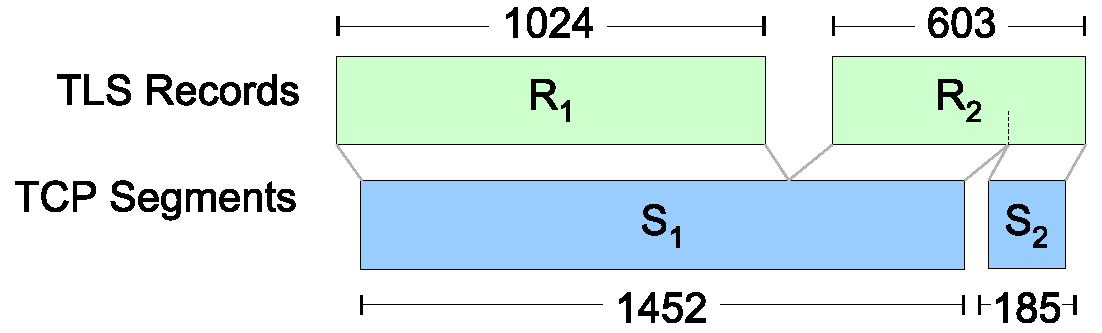
\includegraphics[scale=0.50]{fig/mfl_example}
    \caption{Fragmentação da mensagem \tlsHsC}
    \label{fig:mfl_example}
\end{figure}


\begin{table}[ht]
    \begin{center}
    \caption{\emph{Handshake} com registros limitados a 1024 bytes}
    \label{tab:mfl_run1}
	\begin{tabular}{@{}rclrl@{}} \toprule
%Time (s) & Direction & \multicolumn{2}{c}{TCP} & TLS Records [length] \\ \cmidrule(lr){3-4}
%         & C $\longleftrightarrow$ S &  Flags & Length & \\ \midrule
\tlsFlowHeader \\ \midrule
0.000000 & $\longrightarrow$ & SYN      &	& \\
\altrowcolor
0.028681 & $\longleftarrow$  & SYN, ACK &	& \\
0.028835 & $\longrightarrow$ & ACK      &	& \\
0.031536 & $\longrightarrow$ &		&    57 & Client Hello [52] \\
\altrowcolor
0.072442 & $\longleftarrow$  &		&    86 & Server Hello [81] \\
0.072600 & $\longrightarrow$ & ACK      &	& \\
\altrowcolor
0.096442 & $\longleftarrow$  &		&  1452 & Certificate R1 [1024], \\
\altrowcolor
	 &		     &	        &	& \hl{Certificate R2a} [418/603] \\
0.096567 & $\longrightarrow$ & ACK      &	& \\
\altrowcolor
0.096637 & $\longleftarrow$  &		&   185 & \hl{Certificate R2b} [185/603] \\
0.096708 & $\longrightarrow$ & ACK      &	& \\
\altrowcolor
0.143681 & $\longleftarrow$  &		&     9 & Server Hello Done [4] \\
0.143837 & $\longrightarrow$ & ACK      &	& \\
0.154354 & $\longrightarrow$ &		&   186 & Client Key Exchange [134], \\
	 &		     &		&	& Change Cipher Spec [1], \\
	 &		     &		&	& Finished [36] \\
\altrowcolor
0.328340 & $\longleftarrow$  & ACK      &	& \\
\altrowcolor
0.423803 & $\longleftarrow$  &		&     6 & Change Cipher Spec  [1] \\
0.466072 & $\longrightarrow$ & ACK      &	& \\
\altrowcolor
0.496468 & $\longleftarrow$  &		&    41 & Finished [36] \\
0.497304 & $\longrightarrow$ & ACK      &	& \\
0.500684 & $\longrightarrow$ &		&    27 & Alert - Close Notify [22] \\
0.500964 & $\longrightarrow$ & FIN, ACK &	& \\
\altrowcolor
0.532371 & $\longleftarrow$  & ACK      &	& \\
\altrowcolor
0.548267 & $\longleftarrow$  & FIN, ACK &	& \\
0.548366 & $\longrightarrow$ & ACK      &	& \\ \bottomrule
	\end{tabular}
    \end{center}
\end{table}

\subsubsection{Segunda conexão (\emph{resumed handshake})}

A segunda conexão realizada logo em seguida e cujos resultados estão sintetizados
na Tabela~\vref{tab:mfl_run2}, comprova duas outras 
funcionalidades:

\begin{enumerate}
\item Que após a restauração da sessão o limite do tamanho de cada registro 
voltou a ser o valor negociado na sessão anterior (1024); e
\item Esse limite é efetivo após o \emph{handshake}, como fica evidente pelo 
desmembramento da resposta (\emph{Application Data}) em 8 registros.
\end{enumerate}

\begin{table}[ht]
    \begin{center}
    \caption{Conexão TLS com registros limitados a 1024 bytes}
    \label{tab:mfl_run2}
	\begin{tabular}{@{}rclrl@{}} \toprule
%Time (s) & Direction & \multicolumn{2}{c}{TCP} & TLS Records [length] \\ \cmidrule(lr){3-4}
%         & C $\longleftrightarrow$ S &  Flags & Length & \\ \midrule
\tlsFlowHeader \\ \midrule
0.501275 & $\longrightarrow$ & SYN      &	& \\
\altrowcolor
0.533568 & $\longleftarrow$  & SYN, ACK &       & \\
0.533708 & $\longrightarrow$ & ACK      &       & \\
0.534627 & $\longrightarrow$ &          &    89 & Client Hello [84] \\
\altrowcolor
0.658061 & $\longleftarrow$  &          &    79 & Server Hello [74] \\
0.659113 & $\longrightarrow$ & ACK      &       & \\
\altrowcolor
0.691062 & $\longleftarrow$  &          &    47 & Change Cipher Spec [1], \\
\altrowcolor
         &                   &          &       & Finished [36] \\
0.696049 & $\longrightarrow$ & ACK      &       & \\
0.697457 & $\longrightarrow$ &          &    47 & Change Cipher Spec [1], \\
         &                   &          &       & Finished [36] \\
\altrowcolor
0.926678 & $\longleftarrow$  & ACK      &       & \\
8.144505 & $\longrightarrow$ &          &    46 & Application Data [41] \\
\altrowcolor
8.260117 & $\longleftarrow$  &          &  1049 & Application Data R1 [1044] \\
\altrowcolor
8.286967 & $\longleftarrow$  &          &  1452 & Application Data R2 [1044], \\
\altrowcolor
         &                   &          &       & \hl{Application Data R3a} [398/1044] \\
8.287067 & $\longrightarrow$ & ACK      &       & \\
\altrowcolor
8.291990 & $\longleftarrow$  &          &   646 & \hl{Application Data R3b} [646/1044] \\
\altrowcolor
8.308943 & $\longleftarrow$  &          &  1452 & Application Data R4 [1044], \\
         &                   &          &       & \hl{Application Data R5a} [398/1044] \\
8.309037 & $\longrightarrow$ & ACK      &       & \\
\altrowcolor
8.314126 & $\longleftarrow$  &          &   646 & \hl{Application Data R5b} [646/1044] \\
\altrowcolor
8.338292 & $\longleftarrow$  &          &  1452 & Application Data R6 [1044], \\
\altrowcolor
         &                   &          &       & \hl{Application Data R7a} [398/1044] \\
8.338386 & $\longrightarrow$ & ACK      &       & \\
\altrowcolor
8.343465 & $\longleftarrow$  &          &   646 & \hl{Application Data R7b} [646/1044] \\
\altrowcolor
8.377197 & $\longleftarrow$  &          &   832 & Application Data R8 [827] \\
8.377291 & $\longrightarrow$ & ACK      &       & \\
8.379235 & $\longrightarrow$ &          &    27 & Alert - Close Notify [22] \\
8.379346 & $\longrightarrow$ & FIN, ACK &       & \\
\altrowcolor
8.456271 & $\longleftarrow$  & ACK      &       & \\ \bottomrule
	\end{tabular}
    \end{center}
\end{table}


%%%%%%%%%%%%%%%%%%%%%%%%%%%%%%%%%%%%%%%%%%%%%
%% Capítulo 2 - Client Certificate URL
%% Copyright 2006 Eliézio Batista de Oliveira
%%%%%%%%%%%%%%%%%%%%%%%%%%%%%%%%%%%%%%%%%%%%%

\section{\acl{CCU}}

\subsection{Especificação}

\begin{lstlisting}[caption={Definição do novo tipo de mensagem de \emph{handshake} \tlsHsCu}]
   enum { 
       ..., certificate_url(21), ..., 
       (255) 
   } HandshakeType;
\end{lstlisting}

\begin{lstlisting}[caption={RFC 3546, trecho da seção 3.3}]
After negotiation of the use of client certificate URLs has been 
successfully completed (by exchanging hellos including 
"client_certificate_url" extensions), clients MAY send a 
"CertificateURL" message in place of a "Certificate" message: 
 
   struct { 
       CertChainType type; 
       URLAndOptionalHash url_and_hash_list<1..2^16-1>; 
   } CertificateURL; 
 
   enum { 
       individual_certs(0), pkipath(1), (255) 
   } CertChainType; 
 
   struct { 
       opaque url<1..2^16-1>; 
       Boolean hash_present; 
       select (hash_present) { 
           case false: struct {}; 
           case true: SHA1Hash; 
       } hash; 
   } URLAndOptionalHash; 
 
   enum { 
       false(0), true(1) 
   } Boolean; 
 
   opaque SHA1Hash[20]; 
 
Here "url_and_hash_list" contains a sequence of URLs and optional 
hashes. 
 
When X.509 certificates are used, there are two possibilities: 
 
-  if CertificateURL.type is "individual_certs", each URL refers to 
   a single DER-encoded X.509v3 certificate, with the URL for the 
   client's certificate first, or 
 
-  if CertificateURL.type is "pkipath", the list contains a single 
   URL referring to a DER-encoded certificate chain, using the type 
   PkiPath described in Section 8.
\end{lstlisting}

\subsection{Divergências}

\begin{enumerate}
\item Os certificados individuais podem estar tanto no formato \acs{PEM} quanto 
\acs{DER} (oficial). Foi implementada uma heurística simples para identificar 
o formato;

\item A aplicação servidora não está exigindo que o tipo \acs{MIME} indicado na 
resposta HTTP seja \verb|application/pkix-pkipath|, como dita a 
especificação.
\end{enumerate}

\subsection{API Estendida}

\begin{lstlisting}[language=C,%
		    emph={tlsx_cert_chain_empty,tlsx_cert_chain_add,%
		    TLSX_set_certificate_chain,TLSX_CTX_set_certificate_fetcher_callback},%
		    caption={API Estendida para a extensão \acs{CCU}}]
/* ----- Client Side ----- */
void tlsx_cert_chain_empty (
    CERTIFICATE_CHAIN *cert_chain 
);

int tlsx_cert_chain_add (
    CERTIFICATE_CHAIN *cert_chain,
    int cert_type,    /* TLSX_CERT_CHAIN_TYPE_INDIVIDUAL or
                         TLSX_CERT_CHAIN_TYPE_PKIPATH */
    const char *url,
    const unsigned char *sha1hash  /* optional (may be NULL) */ 
);

void TLSX_set_certificate_chain (
    SSL *ssl,
    const CERTIFICATE_CHAIN *cert_chain 
);

/* ----- Server Side ----- */
void TLSX_CTX_set_certificate_fetcher_callback (
    SSL_CTX *ctx,
    int (*cb) (
        SSL *ssl,
        void *uarg,
        const char *url, 
        unsigned char **data,
        unsigned int *data_len
    ),
    void *uarg
);
\end{lstlisting}

\subsection{Implementação}

Como a aplicação servidora, ao aceitar essa extensão, assume a 
responsabilidade de obter a cadeia de certificados do cliente, fez-se necessário 
embutir esse mecanismo na aplicação \verb|s_server|. Optou-se pela criação de um 
novo módulo de nome \textit{``wget.c''} que, através da biblioteca \emph{open source} \emph{libcurl}
\cite{Libcurl} implementa um cliente \acs{HTTP} genérico. O pacote de 
desenvolvimento desta biblioteca (\verb|libcurl3-dev|, versão 7.14.0, no ambiente Linux de
testes) deve estar previamente instalado na máquina para \emph{build} da aplicação 
\verb|s_server|.

A geração dos certificados individuais em formato \acs{DER} (\acs{ASN1} binário) a partir 
do formato \acs{PEM} (ASCII Base64) é trivialmente realizada através do comando:

\begin{lstlisting}[caption={Conversão de certificados para o formato \acs{DER}}]
openssl x509 -in cert.pem -out cert.der -outform DER
\end{lstlisting}

Como o formato denominado PKIPATH ainda não é nativamente suportado 
pelo OpenSSL e como também não se encontrou nenhuma ferramenta genérica 
que o suportasse, foi necessária a criação de uma pequena aplicação em Java 1.4 
para realizar essa tarefa (ver Apêndice \vref{chap:MkPkiPath}).

A configuração do servidor \acs{HTTP} (Apache) foi modificada para que o tipo 
\verb|application/pkix-pkipath| seja retornado para os arquivos com extensão  
\texttt{``.pki''}.

\begin{description}[\breaklabel\setlabelstyle{\ttfamily}]

\item[s3\_clnt.c::ssl3\_connect]
	A máquina de estados foi modificada no tratamento do estado 
	\verb|SSL3_ST_CW_CERT_A| onde se decide se a nova mensagem \tlsHsCu 
	será enviada no lugar da \tlsHsC ou não.

\item[s3\_srvr.c::ssl3\_get\_client\_certificate]
	Passou a aceitar e processar a mensagem \tlsHsCu caso tenha sido 
	acordada no estágio inicial do \emph{handshake}. Toda a decodificação dessa nova 
	mensagem está embutida nesta função, delegando apenas a recuperação 
	dos certificados para as funções \verb|tlsx_retrieve_certificate| e 
	\verb|tlsx_retrieve_pkipath| conforme o caso.

\end{description}

\subsection{Testes de Conformidade}

Precisou-se, primeiramente, configurar a aplicação servidora para exibir a 
autenticação do cliente, passando a acioná-la como se segue:

\begin{lstlisting}[caption={Chamada da \texttt{s\_server.sh} para forçar a autenticação do cliente}]
./s_server.sh -Verify 2
\end{lstlisting}

A sintaxe usada na aplicação cliente para exercitar essa extensão foi:

\begin{lstlisting}[caption={Chamada da \texttt{s\_client.sh} para teste da extensão \acs{CCU}}]
./s_client.sh -tlsx_cert_url http://localhost/certs/client.crt \
    -key client.key
\end{lstlisting}

Para capturar também o tráfego \acs{HTTP} entre a aplicação \verb|s_server| e o servidor 
Apache, a chamada do \emph{tethereal} foi modificada para:

\begin{lstlisting}[caption={Chamada do \texttt{tethereal} para capturar tráfegos TLS e HTTP}]
tethereal -i lo -V -x port 443 or port 80
\end{lstlisting}

\subsubsection{Resultado do teste com certificados individuais}

Novamente esbarramos em uma limitação do \emph{tethereal} que não foi capaz de 
decodificar propriamente a nova mensagem \tlsHsCu, que a identificou 
erroneamente como \emph{Encrypted Handshake Message}. Mas é possível comprovar a 
correção da implementação conferindo diretamente a seqüência de bytes do 
registro correspondente a essa nova mensagem, que se encontra destacada na 
listagem a seguir:

\begin{lstlisting}[caption={Mensagem \tlsHsCu}]
Secure Socket Layer 
  TLS Record Layer: Handshake Protocol: Encrypted Handshake Message 
    Content Type: Handshake (22) 
    Version: TLS 1.0 (0x0301) 
    Length: |43|
    Handshake Protocol: Encrypted Handshake Message 
  TLS Record Layer: Handshake Protocol: Client Key Exchange 
    Content Type: Handshake (22) 
    Version: TLS 1.0 (0x0301) 
    Length: 134 
    Handshake Protocol: Client Key Exchange 
      Handshake Type: Client Key Exchange (16) 
      Length: 130 
  TLS Record Layer: Handshake Protocol: Certificate Verify 
    Content Type: Handshake (22) 
    Version: TLS 1.0 (0x0301) 
    Length: 134 
    Handshake Protocol: Certificate Verify 
      Handshake Type: Certificate Verify (15) 
      Length: 130 
  TLS Record Layer: Change Cipher Spec Protocol: Change Cipher Spec 
    Content Type: Change Cipher Spec (20) 
    Version: TLS 1.0 (0x0301) 
    Length: 1 
    Change Cipher Spec Message 
  TLS Record Layer: Handshake Protocol: Encrypted Handshake Message 
    Content Type: Handshake (22) 
    Version: TLS 1.0 (0x0301) 
    Length: 36 
    Handshake Protocol: Encrypted Handshake Message 
 
0000  00 00 00 00 00 00 00 00 00 00 00 00 08 00 45 00   ..............E. 
0010  01 9d ac cf 40 00 40 06 8e 89 7f 00 00 01 7f 00   ....@.@......... 
0020  00 01 c7 bb 01 bb fb 40 02 02 fb b0 f8 01 50 18   .......@......P. 
0030  7f ff d3 25 00 00 16 03 01 |00 2b 15 00 00 27 00|   |...%......+...'.|
0040  |00 24 00 21 68 74 74 70 3a 2f 2f 6c 6f 63 61 6c|   |.$.!http://local|
0050  |68 6f 73 74 2f 63 65 72 74 73 2f 63 6c 69 65 6e|   |host/certs/clien|
0060  |74 2e 63 72 74 00| 16 03 01 00 86 10 00 00 82 00   |t.crt.|..........
0070  80 82 56 c1 53 4a 26 be f1 23 dd 3a 9d 76 19 8c   ..V.SJ&..#.:.v..
0080  ac 0e d0 e1 72 a3 0d 13 b0 59 cd 35 82 e0 ee 23   ....r....Y.5...#
0090  26 8e d7 61 71 09 1d 46 bd 01 86 a8 8b 57 0f e9   &..aq..F.....W..
                          ....... 
0180  01 01 16 03 01 00 24 7e c1 60 17 68 94 44 ae dd   ......$~.`.h.D..
0190  1c 90 2c 40 52 28 42 54 4b 25 3c 9b d0 92 68 67   ..,@R(BTK%<...hg
01a0  d1 ca 9e 6c 13 62 0e d3 ed ae 51                  ...l.b....
\end{lstlisting}

\begin{lstlisting}[caption={Solicitação HTTP enviada pela aplicação \texttt{s\_server}}]
Hypertext Transfer Protocol 
  GET /certs/client.crt HTTP/1.1\r\n 
    Request Method: GET 
    Request URI: /certs/client.crt 
    Request Version: HTTP/1.1 
  Host: localhost\r\n 
  Accept: */*\r\n 
  \r\n
\end{lstlisting}

\begin{lstlisting}[caption={Início (cabeçalho) da resposta HTTP enviada pelo servidor para a aplicação \texttt{s\_server}}]
Hypertext Transfer Protocol 
  HTTP/1.1 200 OK\r\n 
    Request Version: HTTP/1.1 
    Response Code: 200 
  Date: Thu, 05 Jan 2006 17:32:37 GMT\r\n 
  Server: Apache/2.0.54 (Ubuntu) DAV/2 SVN/1.2.0 mod_python/3.1.3 Python/2.4.2 PHP/4.4.0-3 mod_ruby/1.2.4 Ruby/1.8.3(2005-06-23)\r\n 
  Last-Modified: Thu, 05 Jan 2006 17:01:44 GMT\r\n 
  ETag: "240f2-b66-7cbc2e00"\r\n 
  Accept-Ranges: bytes\r\n 
  Content-Length: 2918\r\n 
  Content-Type: application/x-x509-ca-cert\r\n 
  \r\n
\end{lstlisting}

\subsubsection{Resultado do teste com PKIPATH}

A sintaxe usada para aplicação cliente foi modificada para:

\begin{lstlisting}
./s_client.sh -tlsx_pkipath_url http://localhost/certs/certs.pki \ 
    -key client.key
\end{lstlisting}

Valem as mesmas considerações feitas para o teste anterior quanto à análise dos 
dados capturados pelo \emph{tethereal}.

\begin{lstlisting}[caption={Mensagem \tlsHsCu}]
Secure Socket Layer 
  TLS Record Layer: Handshake Protocol: Encrypted Handshake Message 
    Content Type: Handshake (22) 
    Version: TLS 1.0 (0x0301) 
    Length: |42| 
    Handshake Protocol: Encrypted Handshake Message 
  TLS Record Layer: Handshake Protocol: Client Key Exchange 
    Content Type: Handshake (22) 
    Version: TLS 1.0 (0x0301) 
    Length: 134 
    Handshake Protocol: Client Key Exchange 
      Handshake Type: Client Key Exchange (16) 
      Length: 130 
  TLS Record Layer: Handshake Protocol: Certificate Verify 
    Content Type: Handshake (22) 
    Version: TLS 1.0 (0x0301) 
    Length: 134 
    Handshake Protocol: Certificate Verify 
      Handshake Type: Certificate Verify (15) 
      Length: 130 
  TLS Record Layer: Change Cipher Spec Protocol: Change Cipher Spec 
    Content Type: Change Cipher Spec (20) 
    Version: TLS 1.0 (0x0301) 
    Length: 1 
    Change Cipher Spec Message 
  TLS Record Layer: Handshake Protocol: Encrypted Handshake Message 
    Content Type: Handshake (22) 
    Version: TLS 1.0 (0x0301) 
    Length: 36 
    Handshake Protocol: Encrypted Handshake Message 

0000  00 00 00 00 00 00 00 00 00 00 00 00 08 00 45 00   ..............E. 
0010  01 9c 6a 03 40 00 40 06 d1 56 7f 00 00 01 7f 00   ..j.@.@..V...... 
0020  00 01 cd 70 01 bb 21 39 b1 cc 20 ef 7e 63 50 18   ...p..!9.. .~cP. 
0030  7f ff d2 22 00 00 16 03 01 |00 2a 15 00 00 26 01|   ...".....|.*...&.|
0040  |00 23 00 20 68 74 74 70 3a 2f 2f 6c 6f 63 61 6c|   |.#. http://local|
0050  |68 6f 73 74 2f 63 65 72 74 73 2f 63 65 72 74 73|   |host/certs/certs|
0060  |2e 70 6b 69 00| 16 03 01 00 86 10 00 00 82 00 80   |.pki.|...........
0070  7c fb e4 c7 8a 27 ef 23 2d 18 f8 be f2 97 d1 34   .....'.#-......4
0080  30 b0 a3 4b 1f d8 b5 8e 49 d5 a6 eb 3e ea af 6d   0..K....I...>..m
0090  ae a1 0d 94 cb 66 89 b4 74 d2 86 5d 64 80 c0 96   .....f..t..]d...
                          ....... 
0180  01 16 03 01 00 24 7e bc d4 51 8f a9 95 33 b6 0c   .....$~..Q...3..
0190  0b c2 db 9b 8d cc 56 28 81 14 a0 74 35 36 3e 8b   ......V(...t56>.
01a0  22 9c f1 f1 0d d3 3e 0f fe 3b                     ".....>..
\end{lstlisting}

\begin{lstlisting}[caption={Solicitação HTTP enviada pela aplicação \texttt{s\_server}}]
Hypertext Transfer Protocol 
  GET /certs/certs.pki HTTP/1.1\r\n 
    Request Method: GET 
    Request URI: /certs/certs.pki 
    Request Version: HTTP/1.1 
  Host: localhost\r\n 
  Accept: */*\r\n 
  \r\n
\end{lstlisting}

\begin{lstlisting}[caption={Início (cabeçalho) da resposta HTTP enviada pelo servidor para a aplicação \texttt{s\_server}}]
Hypertext Transfer Protocol 
  HTTP/1.1 200 OK\r\n 
    Request Version: HTTP/1.1 
    Response Code: 200 
  Date: Thu, 05 Jan 2006 17:49:30 GMT\r\n 
  Server: Apache/2.0.54 (Ubuntu) DAV/2 SVN/1.2.0 mod_python/3.1.3 Python/2.4.2 PHP/4.4.0-3 mod_ruby/1.2.4 Ruby/1.8.3(2005-06-23)\r\n 
  Last-Modified: Thu, 05 Jan 2006 16:42:45 GMT\r\n 
  ETag: "240f0-654-38d86b40"\r\n 
  Accept-Ranges: bytes\r\n 
  Content-Length: 1620\r\n 
  Content-Type: application/pkix-pkipath\r\n 
  \r\n
\end{lstlisting}


%%%%%%%%%%%%%%%%%%%%%%%%%%%%%%%%%%%%%%%%%%%%%
%% Capítulo 2 - Truncated HMAC
%% Copyright 2006 Eliézio Batista de Oliveira
%%%%%%%%%%%%%%%%%%%%%%%%%%%%%%%%%%%%%%%%%%%%%

\section{\acl{TMAC}}

\subsection{Especificação}

\begin{lstlisting}[caption={RFC 3546, trecho da seção 3.5}]
The "extension_data" field of this extension SHALL be empty.
\end{lstlisting}

\subsection{API Estendida}

\begin{lstlisting}[language=C,emph={TLSX_enable_truncated_hmac},caption={API Estendida para a extensão \acs{TMAC}}]
void TLSX_enable_truncated_hmac (
    SSL *ssl
);
\end{lstlisting}

\subsection{Divergências}
Nenhuma.

\subsection{Implementação}

\begin{description}[\breaklabel\setlabelstyle{\ttfamily}]

\item[s3\_clnt.c::ssl3\_connect]
	A máquina de estados foi modificada no tratamento do estado \verb|SSL_ST_OK|
	quando o parâmetro \verb|tlsx_truncated_hmac| é efetivado se assim foi 
	acordado com o servidor.

\item[s3\_pkt.c::ssl3\_get\_record]
	Modificada para reduzir o tamanho do \acl{HMAC} da mensagem a ser 
	validada para \verb|TLSX_TRUNCATED_HMAC_SIZE| (10) se assim foi acordado.

\item[s3\_pkt.c::do\_ssl3\_write]
	Modificada para reduzir o tamanho do \acl{HMAC} da mensagem a ser escrita 
	para \verb|TLSX_TRUNCATED_HMAC_SIZE| (10) se assim foi acordado.

\item[s3\_srvr.c::ssl3\_accept]
	No estado \verb|SSL_ST_OK| quando o parâmetro \verb|tlsx_truncated_hmac| é 
	efetivado se assim foi acordado com o cliente;

\end{description}

\subsection{Testes de Conformidade}

Além de demonstrar a redução no tamanho do \acs{HMAC}, os testes foram 
projetados para comprovar que essa redução só é efetiva após a conclusão do 
\emph{handshake} (não afetando a mensagem \tlsHsF, portanto) e que esse parâmetro 
volta a ser efetivo após a restauração da sessão.

A sintaxe usada na chamada do cliente \verb|s_client| foi:

\begin{lstlisting}[caption={}]
./s_client.sh -tlsx_truncated_hmac
\end{lstlisting}

Duas conexões TLS foram estabelecidas com o seguinte diálogo entre as 
aplicações \verb|s_client| e \verb|s_server|:

\begin{table}[hbtp]
    \begin{center}
    \caption{Diálogo entre as aplicações \texttt{s\_client} e \texttt{s\_server} para testar a eficácia da extensão \acs{TMAC}}
    \label{tab:thmac_clnt_srvr_diag}
	\begin{tabular}{@{}ll@{}} \toprule
	\textbf{\texttt{\sf s\_client}} & \textbf{\texttt{\sf s\_server}} \\ \midrule
request 1 &		\\
	  & response 1	\\
N	  &		\\
request 2 &		\\
	  & response 2	\\
Q	  &		\\ \bottomrule
	\end{tabular}
    \end{center}
\end{table}

Todo o tráfego dessas conexões foi capturado e encontra-se sintetizado nas 
Tabelas~\ref{tab:tmac_run1} e \ref{tab:tmac_run2}:

\begin{table}[ht]
    \begin{center}
    \caption{Primeira conexão (nova): Registros com \acs{HMAC} reduzido}
    \label{tab:tmac_run1}
	\begin{tabular}{@{}rclrl@{}} \toprule
%Time (s) & Direction & \multicolumn{2}{c}{TCP} & TLS Records [length] \\ \cmidrule(lr){3-4}
%         & C $\longleftrightarrow$ S &  Flags & Length & \\ \midrule
\tlsFlowHeader \\ \midrule
0.000000 & $\longrightarrow$ & SYN	&	& \\
\altrowcolor
0.145307 & $\longleftarrow$  & SYN, ACK	&	& \\
0.145435 & $\longrightarrow$ & ACK	&	& \\
0.148974 & $\longrightarrow$ &		&    56 & Client Hello [51] \\
\altrowcolor
1.897516 & $\longleftarrow$  &		&  1452 & Server Hello [80], \\
\altrowcolor
	 &		     &		&	& Certificate [1362/1627] \\
0.414415 & $\longrightarrow$ & ACK	&	& \\
\altrowcolor
0.415191 & $\longleftarrow$  &		&   274 & Certificate [265/1627], \\
	 &		     &		&	& Server Hello Done [4] \\
0.415762 & $\longrightarrow$ & ACK	&	& \\
0.428106 & $\longrightarrow$ &		&   186 & Client Key Exchange [134], \\
	 &		     &		&	& Change Cipher Spec [1], \\
	 &		     &		&	& Finished [36] \\
\altrowcolor
0.627651 & $\longleftarrow$  &		&    47 & Change Cipher Spec [1], \\
\altrowcolor
	 &		     &		&	& Finished [36] \\
0.667665 & $\longrightarrow$ & ACK	&	& \\
3.680601 & $\longrightarrow$ &		&    25 & Application Data [\hl{20}] \\
\altrowcolor
3.856378 & $\longleftarrow$  & ACK	&	& \\
\altrowcolor
9.955240 & $\longleftarrow$  &		&    26 & Application Data [\hl{21}] \\
9.955423 & $\longrightarrow$ & ACK	&	& \\
13.803550 & $\longrightarrow$ &		&    17 & Alert - Close Notify [12] \\
13.803895 & $\longrightarrow$ & FIN, ACK&	& \\
\altrowcolor
13.842239 & $\longleftarrow$  & ACK	&	& \\
\altrowcolor
13.851260 & $\longleftarrow$  & FIN, ACK&	& \\
13.851370 & $\longrightarrow$ & ACK	&	& \\ \midrule
	\end{tabular}
    \end{center}
\end{table}

\begin{table}[ht]
    \begin{center}
    \caption{Primeira conexão (restaurada): Registros com \acs{HMAC} reduzido}
    \label{tab:tmac_run2}
	\begin{tabular}{@{}rclrl@{}} \toprule
%Time (s) & Direction & \multicolumn{2}{c}{TCP} & TLS Records [length] \\ \cmidrule(lr){3-4}
%         & C $\longleftrightarrow$ S &  Flags & Length & \\ \midrule
\tlsFlowHeader \\ \midrule
13.804240 & $\longrightarrow$ & SYN	&	& \\
\altrowcolor
13.845121 & $\longleftarrow$  & SYN, ACK&	& \\
13.845296 & $\longrightarrow$ & ACK	&	& \\
13.846581 & $\longrightarrow$ &		&    88 & Client Hello [83] \\
\altrowcolor
13.956312 & $\longleftarrow$  &		&   126 & Server Hello [74], \\
	  &		      &		&	& Change Cipher Spec [1], \\
	  &		      &		&	& Finished [36] \\
13.957341 & $\longrightarrow$ & ACK	&	& \\
13.959072 & $\longrightarrow$ &		&    47 & Change Cipher Spec [1], \\
	  &		      &		&	& Finished [36] \\
\altrowcolor
14.088635 & $\longleftarrow$  &	ACK	&	& \\
17.725468 & $\longrightarrow$ &		&    25 & Application Data [\hl{20}] \\
\altrowcolor
17.902308 & $\longleftarrow$  & ACK	&	& \\
\altrowcolor
21.159691 & $\longleftarrow$  &		&    26 & Application Data [\hl{21}] \\
21.199546 & $\longrightarrow$ & ACK	&	& \\
22.834441 & $\longrightarrow$ &		&    17 & Alert - Close Notify [12] \\
22.834557 & $\longrightarrow$ & FIN, ACK&	& \\ \bottomrule
	\end{tabular}
    \end{center}
\end{table}

\begin{lstlisting}[caption={Detalhe do \tlsHsCh estendido}]
Secure Socket Layer
  SSL Record Layer: Handshake Protocol: Client Hello 
    Content Type: Handshake (22) 
    Version: TLS 1.0 (0x0301) 
    Length: 51 
    Handshake Protocol: Client Hello 
      Handshake Type: Client Hello (1) 
      Length: 47 
      Version: TLS 1.0 (0x0301) 
      Random.gmt_unix_time: Jan  6, 2006 09:10:53.000000000 
      Random.bytes 
      Session ID Length: 0 
      Cipher Suites Length: 2 
      Cipher Suites (1 suite) 
	Cipher Suite: TLS_RSA_WITH_RC4_128_SHA (0x0005) 
      Compression Methods Length: 1 
      Compression Methods (1 method) 
	Compression Method: null (0) 
      Extensions Length: 4 
      Extension: truncated_hmac 
	Type: truncated_hmac (|0x0004|) 
	Length: |0| 
	Data (0 bytes)
\end{lstlisting}


%%%%%%%%%%%%%%%%%%%%%%%%%%%%%%%%%%%%%%%%%%%%%
%% Capítulo 2 - Trusted CA Indication
%% Copyright 2006 Eliézio Batista de Oliveira
%%%%%%%%%%%%%%%%%%%%%%%%%%%%%%%%%%%%%%%%%%%%%

\section{\acl{TCI}}

\subsection{Especificação}

\begin{lstlisting}[caption={RFC 3546, trecho da seção 3.4}]
The "extension_data" field of this extension SHALL contain 
"TrustedAuthorities" where: 
 
   struct { 
       TrustedAuthority trusted_authorities_list<0..2^16-1>; 
   } TrustedAuthorities; 
 
   struct { 
       IdentifierType identifier_type; 
       select (identifier_type) { 
           case pre_agreed: struct {}; 
           case key_sha1_hash: SHA1Hash; 
           case x509_name: DistinguishedName; 
           case cert_sha1_hash: SHA1Hash; 
       } identifier; 
   } TrustedAuthority; 
 
   enum { 
       pre_agreed(0), key_sha1_hash(1), x509_name(2), 
       cert_sha1_hash(3), (255) 
   } IdentifierType; 
 
   opaque DistinguishedName<1..2^16-1>; 
 
 
Here "TrustedAuthorities" provides a list of CA root key identifiers 
that the client possesses.  Each CA root key is identified via 
either: 
 
-  "pre_agreed" - no CA root key identity supplied. 
-  "key_sha1_hash" - contains the SHA-1 hash of the CA root key.  For 
   DSA and ECDSA keys, this is the hash of the "subjectPublicKey" 
   value.  For RSA keys, the hash is of the big-endian byte string 
   representation of the modulus without any initial 0-valued bytes. 
   (This copies the key hash formats deployed in other environments.) 
 
-  "x509_name" - contains the DER-encoded X.509 DistinguishedName of 
   the CA. 
 
-  "cert_sha1_hash" - contains the SHA-1 hash of a DER-encoded 
   Certificate containing the CA root key.
\end{lstlisting}

\subsection{API Estendida}

\begin{lstlisting}[language=C,emph={TLSX_set_trusted_ca},caption={API Estendida para a extensão \acs{TCI}}]
void TLSX_set_trusted_ca (
    SSL *ssl,
    int id_type,    /* TLSX_CERT_ID_PRE_AGREED,
		       TLSX_CERT_ID_KEY_SHA1_HASH,
		       TLSX_CERT_ID_X509_NAME, or
		       TLSX_CERT_ID_CERT_SHA1_HASH */
    const char *CAfile,  /* optional */
    const char *CApath   /* optional */
);
\end{lstlisting}

Essa função associa ao objeto \verb|SSL| uma lista de IDs de todos os certificados 
encontrados no diretório indicado por \verb|CApath| cujo nome base (sem diretório) 
adere ao padrão utilizado pelo OpenSSL para certificados de \acsp{CA}, ou seja, 
segue o formato \texttt{``hhhhhhhh.d''}, onde \texttt{``hhhhhhhh''} é uma seqüência de oito 
dígitos hexadecimais e \texttt{``d''} é um dígito decimal. O certificado opcionalmente 
indicado por \verb|CAfile| é também acrescido a esse conjunto. Todos esses 
certificados devem estar em formato \acs{PEM} (Base-64).

\subsection{Divergências}

\begin{enumerate}

\item Não foi possível implementar a parte servidora dessa extensão pois o OpenSSL não permite a configuração de um servidor com múltiplos certificados diferenciados apenas pelo emissor;

\item Como normalmente as aplicações que utilizam o OpenSSL especificam o
\emph{Certificate Store} coletivamente (via \verb|SSL_CTX_load_verify_locations|),
a API estendida obriga a adoção de um mesmo tipo de 
identificador para todos os certificados.

\end{enumerate}

\subsection{Testes de Conformidade}

Como os resultados são bastante semelhantes para os diversos tipos de IDs, 
apresenta-se aqui somente o resultado de teste efetuado com o tipo 
\verb|TLSX_CERT_ID_CERT_SHA1_HASH| com seguinte sintaxe na execução da aplicação 
\verb|s_client|:

\begin{lstlisting}
./s_client.sh -tlsx_trusted_ca_id cert_sha1_hash
\end{lstlisting}

O diretório de trabalho possuía somente um certificado cujo \emph{hash} \acs{SHA1} pôde 
ser obtido diretamente com o comando \verb|sha1sum|:

\begin{lstlisting}[caption={Cálculo do \emph{hash} \acs{SHA1} do certificado do CA}]
ebo@esparta:~/openssl-tlsx$ sha1sum 3ff23a0a.d 
|27399b0a3e46c936852cc3662b90d0e4d8635e78|  3ff23a0a.d
\end{lstlisting}

A equivalência do \emph{hash} obtido com esse comando e o enviado na mensagem 
\tlsHsCh abaixo (destacado em negrito e itálico no final da listagem), 
comprova a correção da implementação desta extensão.

\begin{lstlisting}[caption={Mensagem \tlsHsCh contendo a extensão \acs{TCI}}]
Secure Socket Layer 
  SSL Record Layer: Handshake Protocol: Client Hello 
    Content Type: Handshake (22) 
    Version: TLS 1.0 (0x0301) 
    Length: 72 
    Handshake Protocol: Client Hello 
      Handshake Type: Client Hello (1) 
      Length: 68 
      Version: TLS 1.0 (0x0301) 
      Random.gmt_unix_time: Jan  5, 2006 16:20:24.000000000 
      Random.bytes 
      Session ID Length: 0 
      Cipher Suites Length: 2 
      Cipher Suites (1 suite) 
	Cipher Suite: TLS_RSA_WITH_RC4_128_SHA (0x0005) 
      Compression Methods Length: 1 
      Compression Methods (1 method) 
	Compression Method: null (0) 
      Extensions Length: 25 
      Extension: trusted_ca_keys 
	Type: trusted_ca_keys (|0x0003|) 
	Length: |21| 
	Data (21 bytes) 
 
0000  00 00 00 00 00 00 00 00 00 00 00 00 08 00 45 00   ..............E. 
0010  00 75 22 ee 40 00 40 06 19 93 7f 00 00 01 7f 00   .u".@.@......... 
0020  00 01 c7 a9 01 bb eb ae f5 b1 eb 59 e3 a9 50 18   ...........Y..P. 
0030  7f ff 72 72 00 00 16 03 01 00 48 01 00 00 44 03   ..rr......H...D. 
0040  01 43 bd 63 68 29 5c 97 3f 14 37 d7 76 c0 11 35   .C.ch)\.?.7.v..5 
0050  6e 25 fc bd 6a d8 91 e9 1d b9 2e 85 cf 39 38 56   n%..j........98V 
0060  bb 00 00 02 00 05 01 00 00 19 |00 03 00 15 03 27|   ..........|.....'| 
0070  |39 9b 0a 3e 46 c9 36 85 2c c3 66 2b 90 d0 e4 d8|   |9..>F.6.,.f+....| 
0080  |63 5e 78|                                          |c^x|
\end{lstlisting}


%%%%%%%%%%%%%%%%%%%%%%%%%%%%%%%%%%%%%%%%%%%%%
%% Capítulo 2 - Server Certificate Chain ID
%% Copyright 2006 Eliézio Batista de Oliveira
%%%%%%%%%%%%%%%%%%%%%%%%%%%%%%%%%%%%%%%%%%%%%

\section{\acl{SCCI}}

\subsection{Especificação}

\begin{lstlisting}[caption={Definição (não-oficial) da extensão \acs{SCCI}}]
      enum { 
          ..., certificate_chain(10), (65535) 
      } ExtensionType;
\end{lstlisting}

\begin{lstlisting}[caption={Especificação (não-oficial) da extensão \acs{SCCI}}]
The "extension_data" field of this extension SHALL contain
"CertificateIdentifiers" where: 
  
   struct { 
       CertificateIdentifier certificate_identifiers_list<0..2^16-1>; 
   } CertificateIdentifiers; 
 
CertificateIdentifier has the same definition of TrustedAuthority.
\end{lstlisting}

\subsection{API Estendida}

\begin{lstlisting}[language=C,emph={TLSX_get_cert_chain,TLSX_set_server_cert_chain,TLSX_free_cert_chain},%
		    caption={API Estendida para a extensão \acs{SCCI}}]
/* Client Side */
STACK_OF(X509) *TLSX_get_cert_chain (
  SSL *ssl
);

void TLSX_set_server_cert_chain (
  SSL *ssl,
  STACK_OF(X509) *cert_chain,
  int id_type		/* TLSX_CERT_ID_PRE_AGREED,
			   TLSX_CERT_ID_KEY_SHA1_HASH,
			   TLSX_CERT_ID_X509_NAME, or
			   TLSX_CERT_ID_CERT_SHA1_HASH */
);

void TLSX_free_cert_chain (
  STACK_OF(X509) **chain
);
\end{lstlisting}

A \verb|TSLX_get_cert_chain| deve ser usada em qualquer momento após o 
estabelecimento da conexão TLS, mas antes do fechamento da mesma. Ela 
devolve uma cópia de toda a cadeia de certificados do servidor que
poderá então ser usada na próxima conexão a este 
mesmo servidor. A função \verb|TLSX_set_server_cert_chain| atribui uma referência a 
esta cadeia ao objeto SSL e ativa automaticamente a extensão \acl{SCCI}.

A função \verb|TLSX_free_cert_chain| libera toda a memória utilizada por essa cadeia 
quando não estiver mais sendo referenciada por nenhum objeto SSL. Essa 
referência será anulada quando da destruição do objeto SSL associado ou 
explicitamente através da chamada \verb|TLSX_set_server_cert_chain(ssl, NULL, 0)|.

\subsection{Divergências}
Nenhuma por não haver uma norma oficial.

\subsection{Implementação}

\begin{description}[\breaklabel\setlabelstyle{\ttfamily}]

\item[s3\_both.c::ssl3\_output\_cert\_chain]
	Na versão original criava e serializava toda uma cadeia de certificados 
	diretamente no \emph{buffer} de saída, a partir do certificado final. Foi 
	modificada para construir a cadeia e ao final decidir se esta será 
	serializada ou será inteiramente suprimida, o que ocorrerá somente se as 
	seguintes condições forem atendidas:
	\begin{enumerate}
	    \item O papel da conexão for ``servidor'';
	    \item A extensão \acl{SCCI} tiver sido proposta e aceita;
	    \item Houver uma correspondência integral entre os IDs informados na
	    extensão e os certificados selecionados.
	\end{enumerate}

\item[s3\_clnt.c::ssl3\_get\_server\_certificate]
	Caso a mensagem \tlsHsC oriunda do servidor esteja vazia e a extensão 
	\acl{SCCI} tiver sido acordada, a cadeia de certificados será 
	simplesmente uma cópia da cadeia definida através da função 
	\verb|TLSX_set_server_cert_chain|. Nesse ponto é também incluída essa cadeia 
	no cômputo do \emph{hash} da mensagem \tlsHsF enviada ao final do \emph{handshake}.

\item[s3\_srvr.c::ssl3\_accept]
	Modificada para atualizar o \emph{hash} a ser enviado na mensagem \tlsHsF com 
	toda a cadeia de certificados caso esta tenha sido omitida na 
	\verb|ssl3_output_cert_chain|.

\end{description}

\subsection{Testes de Conformidade}

O teste foi realizado com a seguinte execução da aplicação \verb|s_client|:

\begin{lstlisting}[caption={Chamada da \texttt{s\_client.sh} para o teste da extensão \acs{SCCI}}]
./s_client.sh -tlsx_server_cert_id cert_sha1_hash
\end{lstlisting}

Uma vez acionada, entrou-se com a string \texttt{``n''} para forçar uma segunda 
conexão TLS sem \emph{session resumption}. As mensagens TLS dessa última conexão e 
que foram impactadas por essa extensão encontram-se exibidas a seguir.

\begin{lstlisting}[caption={Mensagem \tlsHsCh com a extensão \acs{SCCI}}]
Secure Socket Layer 
  SSL Record Layer: Handshake Protocol: Client Hello 
    Content Type: Handshake (22) 
    Version: TLS 1.0 (0x0301) 
    Length: 93 
    Handshake Protocol: Client Hello 
      Handshake Type: Client Hello (1) 
      Length: 89 
      Version: TLS 1.0 (0x0301) 
      Random.gmt_unix_time: Jan  6, 2006 15:54:17.000000000 
      Random.bytes 
      Session ID Length: 0 
      Cipher Suites Length: 2 
      Cipher Suites (1 suite) 
	Cipher Suite: TLS_RSA_WITH_RC4_128_SHA (0x0005) 
      Compression Methods Length: 1 
      Compression Methods (1 method) 
	Compression Method: null (0) 
      Extensions Length: 46 
      Extension: Unknown 10 
	Type: Unknown (|0x000a|) 
	Length: |42| 
	Data (42 bytes) 
 
0000  00 c0 49 43 0b 55 00 50 04 aa 26 05 08 00 45 00   ..IC.U.P..&...E. 
0010  00 8a 93 d1 40 00 40 06 c7 5a 0a 04 02 14 c9 2d   ....@.@..Z.....- 
0020  09 fd a1 49 01 bb c6 bc e9 53 a6 d2 a6 84 50 18   ...I.....S....P. 
0030  16 d0 3c 21 00 00 16 03 01 00 5d 01 00 00 59 03   ..<!......]...Y. 
0040  01 43 be ae c9 59 97 28 3d 2c ef 3e d6 73 92 cd   .C...Y.(=,.>.s.. 
0050  6a 83 e0 2f 0b ef b1 d1 46 8d 07 b1 6a f5 58 97   j../....F...j.X. 
0060  a9 00 00 02 00 05 01 00 00 2e |00 0a 00 2a 03 0d|   ..........|...*..| 
0070  |5c 3c bb 76 60 b4 36 9b a3 11 16 db 87 bd c0 81|   |\<.v`.6.........| 
0080  |c1 14 da 03 27 39 9b 0a 3e 46 c9 36 85 2c c3 66|   |....'9..>F.6.,.f| 
0090  |2b 90 d0 e4 d8 63 5e 78|                           |+....c^x|
\end{lstlisting}

\begin{lstlisting}[caption={Resposta do servidor com destaque para a mensagem \tlsHsC vazia}]
Secure Socket Layer 
  TLS Record Layer: Handshake Protocol: Server Hello 
    Content Type: Handshake (22) 
    Version: TLS 1.0 (0x0301) 
    Length: 80 
    Handshake Protocol: Server Hello 
      Handshake Type: Server Hello (2) 
      Length: 76 
      Version: TLS 1.0 (0x0301) 
      Random.gmt_unix_time: Jan  6, 2006 15:54:09.000000000 
      Random.bytes 
      Session ID Length: 32 
      Session ID (32 bytes) 
      Cipher Suite: TLS_RSA_WITH_RC4_128_SHA (0x0005) 
      Compression Method: null (0) 
      Extensions Length: 4 
      Extension: Unknown 10 
	Type: Unknown (|0x000a|) 
	Length: |0| 
	Data (0 bytes) 
  TLS Record Layer: Handshake Protocol: |Certificate| 
    Content Type: Handshake (22) 
    Version: TLS 1.0 (0x0301) 
    Length: 7 
    Handshake Protocol: Certificate 
      Handshake Type: Certificate (11) 
      Length: 3 
      Certificates Length: |0| 
  TLS Record Layer: Handshake Protocol: Server Hello Done 
    Content Type: Handshake (22) 
    Version: TLS 1.0 (0x0301) 
    Length: 4 
    Handshake Protocol: Server Hello Done 
      Handshake Type: Server Hello Done (14) 
      Length: 0
\end{lstlisting}



%%%%%%%%%%%%%%%%%%%%%%%%%%%%%%%%%%%%%%%%%%%%%
%% Conclusão e Trabalhos Futuros
%% Copyright 2006 Eliézio Batista de Oliveira
%%%%%%%%%%%%%%%%%%%%%%%%%%%%%%%%%%%%%%%%%%%%%

\chapter{Conclusão e Trabalhos Futuros}

\section{Conclusão}

Apesar da RFC~3546 ter sido publicada há quase três anos, somente agora
tem surgido implementações das extensões propostas, mas mesmo assim parciais.

A versão em desenvolvimento do OpenSSL (0.9.9) já contém uma implementação funcional da
extensão \acl{SNI} que também é contemplada na vindoura versão do \emph{browser} Opera (9.0)
e na pilha GnuTLS.

As demais extensões, todas voltadas para sistemas embutidos, tem recebido pouca ou quase nenhuma
atenção dos desenvolvedores de \emph{software} \emph{open-source}, assim como de empresas comerciais.

Com base na minha experiência em desenvolvimento de soluções de comunicação, entendo que esse interesse
tem sido atenuado por alguns mitos:

\begin{itemize}

\item De que o ostensivo e contínuo aumento na banda em praticamente todos os meios de comunicação dispensaria a necessidade de esforços para a otimização de protocolos. Essa expectativa não procede pois o aumento na demanda tem sido ainda mais vertiginoso, principalmente em redes utilizadas por equipamentos móveis;

\item Que o mecanismo de restauração de sessões TLS anularia a aplicabilidade da maioria destas
extensões. De fato, com excessão das extensões \acl{MFL} e \acl{TMAC}, todas as outras cinco só são
aplicáveis em \emph{handshakes} completos.

No entanto, ao contrário do muitos supõem, em geral as sessões TLS não são mantidas por muito tempo pelos servidores HTTPS -- os maiores beneficiados por este mecanismo -- por causa do espaço em memória que seria necessário para armazená-las em larga escala.
No site \emph{Amazon.com}, por exemplo, as sessões TLS são descartadas após breves 2 minutos!

\end{itemize}

A minha real expectativa é de que a implementação alvo deste projeto possa contribuir efetivamente
para popularizar o uso dessas extensões para um uso mais racional dos recursos disponíveis para
sistemas restritos.

\section{Propostas de Trabalhos Futuros}

\subsection{Tarefas Gerais}

\begin{itemize}

\item Submissão ao \emph{core team} de desenvolvedores do OpenSSL a fim de 
oficializar esta implementação;

\item Replicar a API proposta no nível \texttt{CTX}, visando a consistência com a API 
oficial do OpenSSL;

\item Garantir que as novas implementações são \emph{thread-safe};

\item Incorporação de outras possíveis extensões já definidas pelo \emph{\acs{IETF} TLS 
Working Group} ou que ainda estejam em fase de discussão. Exemplo: a que 
permite a substituição do \acs{SHA1} por algum algoritmo de \emph{hashing} mais 
seguro (SHA-256 ou SHA-512, por exemplo);

\item Implementar estas extensões em uma pilha SSL/TLS voltada para
sistemas embutidos. O candidato mais adequado parece ser o MatrixSSL (\url{http://www.matrixssl.org/}),
principalmente por causa do seu duplo-licenciamento (GPL e comercial);

\item Corrigir o Ethereal para decodificar corretamente a mensagem \tlsHsCu
e ser capaz de desfragmentar registros;

\end{itemize}

\subsection{Extensão \acl{SNI}}

\begin{itemize}

\item Implementar a parte servidora, incluindo as necessárias modificações
no \emph{``mod\_ssl''} (\url{http://httpd.apache.org/docs/2.0/ssl/}) para ativar e configurar os
seus diversos parâmetros.

\end{itemize}

\subsection{Extensão \acl{CCU}}

\begin{itemize}

\item Implementar o \emph{cache} de certificados no servidor;

\item Analisar a possibilidade de usar algum esquema específico em que o
cliente informe somente o contexto (ou \emph{domain}/\emph{realm}) e um
identificador (\emph{serial number}/\emph{username}) e que o servidor seja
capaz de ``montar'' uma \acs{URL} com base nessas informações e em \emph{template}
configurado;

\item Implementar mecanismos que restrinjam o acesso a um conjunto limitado
de provedores de certificados. Visar também minimizar eventuais ataques do
tipo \ac{DoS}.

\end{itemize}

\subsection{Extensão \acl{CSR}}

\begin{itemize}

\item Além de implementar esta extensão, avaliar a possibilidade do uso de
outros protocolos alternativos, tais como \ac{SCVP}, \ac{DCS} e \ac{OCSPX};

\end{itemize}

\subsection{Extensão \acl{SCCI}}

\begin{itemize}

\item Obtenção de um identificador oficial para esta extensão junto a
\acs{IANA}/\acs{IETF} (vide \url{http://www.iana.org/assignments/tls-extensiontype-values});

\item Submissão desta nova extensão ao grupo de trabalho do \acs{IETF}
responsável pelo TLS para uma possível criação de uma \emph{Internet-Draft} e
futuramente de uma RFC;

\end{itemize}



\appendix

%%%%%%%%%%%%%%%%%%%%%%%%%%%%%%%%%%%%%%%%%%%%%
%% Apêndice - Header tlsx.h
%% Copyright 2006 Eliézio Batista de Oliveira
%%%%%%%%%%%%%%%%%%%%%%%%%%%%%%%%%%%%%%%%%%%%%

\chapter{Header ``tlsx.h''}
\lstinputlisting[language=C,numbers=left,basicstyle=\footnotesize\ttfamily,%
				caption={\emph{Header} \texttt{tlsx.h}}]{../code/tlsx.h}
\label{chap:tlsx_h}

%%%%%%%%%%%%%%%%%%%%%%%%%%%%%%%%%%%%%%%%%%%%%
%% Apêndice - Programa MakePkiPath.java
%% Copyright 2006 Eliézio Batista de Oliveira
%%%%%%%%%%%%%%%%%%%%%%%%%%%%%%%%%%%%%%%%%%%%%

\chapter{Programa ``MakePkiPath.java''}
\lstinputlisting[language=Java,caption={Programa \texttt{MakePkiPath.java}}]{../openssl-tlsx/pkipath/MakePkiPath.java}
\label{chap:MkPkiPath}



%%%%%%%%%%%%%%%%%%%%%%%%%%%%%%%%%%%%%%%%%%%%%
%% Bibliografia
%% Copyright 2006 Eliézio Batista de Oliveira
%%%%%%%%%%%%%%%%%%%%%%%%%%%%%%%%%%%%%%%%%%%%%

\bibliographystyle{abnt-num}
\bibliography{bib/biblio}



\end{document}

